% Präambel
\documentclass[12pt,a4paper,oneside, 
liststotoc, 					% Tabellen- und Abbildungsverzeichnis ins Inhaltsverzeichnis
bibtotoc,						% Literaturverzeichnis ins Inhaltsverzeichnis aufnehmen
titlepage, 						% Titlepage-Umgebung statt \maketitle
headsepline, 					% horizontale Linie unter Kolumnentitel
%abstracton,					% Überschrift beim Abstract einschalten, Abstract muss dazu in {abstract}-Umgebung stehen
%DIV11,							% auskommentieren, um den Seitenspiegel zu vergrößern
BCOR6mm,						% Bindekorrektur, die den Seitenspiegel um 6mm nach rechts verschiebt,
english
]{scrreprt}		
\usepackage{ucs} 				% Dokument in utf8-Codierung schreiben und speichern
\usepackage[utf8x]{inputenc} 	% ermöglicht die direkte Eingabe von Umlauten
\usepackage[ngerman]{babel} 	% deutsche Trennungsregeln und Übersetzung der festcodierten Überschriften
\usepackage[T1]{fontenc} 		% Ausgabe aller zeichen in einer T1-Codierung (wichtig für die Ausgabe von Umlauten!)
\usepackage{graphicx}  			% Einbinden von Grafiken erlauben
%\usepackage{amsmath}
%\usepackage{amsfonts}
%\usepackage{amssymb}
\usepackage{mathpazo} 			% Einstellung der verwendeten Schriftarten
\usepackage{textcomp} 			% zum Einsatz von Eurozeichen u. a. Symbolen
\usepackage{listings}			% Datstellung von Quellcode mit den Umgebungen {lstlisting}, \lstinline und \lstinputlisting
\usepackage{xcolor} 			% einfache Verwendung von Farben in nahezu allen Farbmodellen
\usepackage[intoc]{nomencl} 	% zur Erstellung des Abkürzungsberzeichnisses
\usepackage{fancyhdr}			% Zusatzpaket zur Gestaltung von Fuß und Kopfzeilen
\usepackage[htt]{hyphenat} 		%Line break of classnames
\usepackage{tikz}				%AST tree package
\usepackage{fullpage}
\usepackage{calc}
\usetikzlibrary{positioning,shadows,arrows,trees,shapes,fit}		%use the tree part of the package
\usepackage[printonlyused]{acronym}
\usepackage{times}
% -----------------------------------------------------------------------------------------------------------------
% Zum Aktualisieren des Abkürzungsverzeichnisses bitte auf der Kommandozeile folgenden Befehl aufrufen :
%  makeindex Bachelorarbeit.nlo -s nomencl.ist -o Bachelorarbeit.nls
% -----------------------------------------------------------------------------------------------------------------

% Hier die persönlichen Daten eingeben:

\newcommand{\titel}{Validating the Object Calisthenics}
\newcommand{\untertitel}{Evaluation and Prototypical Implementation of Tool Support}
\newcommand{\arbeit}{Student Research Paper}
\newcommand{\studiengang}{Applied Computer Science}
\newcommand{\autor}{Fabian Schwarz-Fritz}
\newcommand{\matrikelnr}{212024979}
\newcommand{\kurs}{TINF11B2}
\newcommand{\firma}{SAP AG, Walldorf}
\newcommand{\abgabe}{\today}
\newcommand{\betreuerdhbw}{Daniel Lindner}
\newcommand{\betreuerfirma}{Soft­ware­schnei­de­rei GmbH, Karls­ru­he}

\newcommand{\jahr}{2014}			% für Angabe im Copyright-Vermerk der Titelseite

% Abkürzungen
\newcommand{\ua}{\mbox{u.\,a.\ }}
\newcommand{\zB}{\mbox{z.\,B.\ }}
\newcommand{\bs}{$\backslash$}

\renewcommand{\nomname}{Abbreviations}

% Code listing configuration: 

\usepackage{listings}
  \usepackage{courier}
 \lstset{
         basicstyle=\footnotesize\ttfamily, % Standardschrift
         %numbers=left,               % Ort der Zeilennummern
         numberstyle=\tiny,          % Stil der Zeilennummern
         %stepnumber=2,               % Abstand zwischen den Zeilennummern
         numbersep=5pt,              % Abstand der Nummern zum Text
         tabsize=2,                  % Groesse von Tabs
         extendedchars=true,         %
         breaklines=true,            % Zeilen werden Umgebrochen
         keywordstyle=\color{red},
    		frame=b,         
 %        keywordstyle=[1]\textbf,    % Stil der Keywords
 %        keywordstyle=[2]\textbf,    %
 %        keywordstyle=[3]\textbf,    %
 %        keywordstyle=[4]\textbf,   \sqrt{\sqrt{}} %
         stringstyle=\color{white}\ttfamily, % Farbe der String
         showspaces=false,           % Leerzeichen anzeigen ?
         showtabs=false,             % Tabs anzeigen ?
         xleftmargin=17pt,
         framexleftmargin=17pt,
         framexrightmargin=5pt,
         framexbottommargin=4pt,
         %backgroundcolor=\color{lightgray},
         showstringspaces=false      % Leerzeichen in Strings anzeigen ?        
 }
 \lstloadlanguages{% Check Dokumentation for further languages ...
         %[Visual]Basic
         %Pascal
         %C
         %C++
         %XML
         %HTML
         Java
 }
    %\DeclareCaptionFont{blue}{\color{blue}} 

  %\captionsetup[lstlisting]{singlelinecheck=false, labelfont={blue}, textfont={blue}}
\usepackage{caption}
\DeclareCaptionFont{white}{\color{white}}
\DeclareCaptionFormat{listing}{\colorbox[cmyk]{0.43, 0.35, 0.35,0.01}{\parbox{\textwidth}{\hspace{15pt}#1#2#3}}}
\captionsetup[lstlisting]{format=listing,labelfont=white,textfont=white, singlelinecheck=false, margin=0pt, font={bf,footnotesize}}

%\tikzstyle{edge from parent bend}=
%[edge from parent path={(\tikzparentnode\tikzparentanchor) |-
%(\tikzchildnode\tikzchildanchor)}]

%\newcommand{\classname}[1]{\texttt{#1}}
%\lstset{numbers=left}
%\lstset{backgroundcolor=\color{white}}
%\lstset{frame=single}
%\lstset{breaklines=true}
%\lstset{morecomment=[l]{//}}


% -------------------------------------------------------------------------------------------
% Definition der Kopf- und Fußzeilen
\setlength{\headsep}{30pt}
\lhead{}								% Kopf links
\chead{}								% Kopf mitte
\rhead{\sffamily{\titel}}				% Kopf rechts
\lfoot{}								% Fuß links
\cfoot{\sffamily{\thepage}}				% Fuß mitte
\rfoot{\sffamily{\autor}}				% Fuß rechts
\renewcommand{\headrulewidth}{0.4pt}	% Liniendicke Kopf
\renewcommand{\footrulewidth}{0.4pt}	% Liniendicke Fuß


%\makenomenclature							% Abkürzungsverzeichnis erstellen
%
% alle Abkürzungen, die in der Bachelorarbeit verwendet werden
\begin{acronym}
	\acro{DIP}{Dependency Inversion Principle}
	\acro{HTML}{Hyper Text Markup Language}
	\acro{UML}{Unified Modelling Language}
	\acro{LSP}{Liskov Substitution Principle}
	\acro{DDD}{Domain Driven Design}
	\acro{LoD}{Law of Demeter}
	\acro{GWT}{Google Web Toolkit}
\end{acronym}
					% Datei mit Abkürzungen laden

% -------------------------------------------------------------------------------------------
%                     Beginn des Dokumenteninhalts
% -------------------------------------------------------------------------------------------
\begin{document}
\selectlanguage{english}					% Sprache englisch
\setcounter{secnumdepth}{3}					% Nummerierungstiefe fürs Inhaltsverzeichnis
\setcounter{tocdepth}{3}
\sffamily									% für die Titelei serifenlose Schrift verwenden

% ------------------------------ Titelei -----------------------------------------------------

\thispagestyle{plain}
\begin{titlepage}
\enlargethispage{4.0cm}
\sffamily 								% Serifenlose Grundschrift für die Titelseite einstellen
				
\begin{flushright}

\includegraphics[scale=2.0]{Bilder/logo_dhbw.jpg}\\[5ex]
\end{flushright}

\begin{center}

\huge{\textsc{\textbf{\titel}}}\\[1.5ex]
\Large{\textbf{\untertitel}}\\[5ex]
\LARGE{\textbf{\arbeit}}\\[2ex]
\normalsize{für die Prüfung zum\\[1ex] Bachelor of Engineering}\\[3ex]
\Large{Studiengang \studiengang}\\[1ex]
\normalsize{Duale Hochschule Baden-Württemberg Karlsruhe}\\[5ex]
von\\[1ex] \autor \\[18ex]


\end{center}

\begin{flushleft}

\begin{tabular}{ll}
Abgabedatum:					& \quad \abgabe \\
Bearbeitungszeitraum:			& \quad 12 Wochen   \\ 
Matrikelnummer, Kurs: 			& \quad \matrikelnr , \kurs \\ 
Ausbildungsfirma:	 			& \quad \firma \\ 
Betreuer der Ausbildungsfirma:  & \quad \betreuerfirma \\ 
Gutachter der Dualen Hochschule: & \quad \betreuerdhbw \\ [5ex]

\end{tabular} 



\small
Copyrightvermerk:\\

Dieses Werk einschließlich seiner Teile ist \textbf{urheberrechtlich geschützt}. Jede Verwertung außerhalb der engen Grenzen des Urheberrechtgesetzes ist ohne Zustimmung des Autors unzulässig und strafbar. Das gilt insbesondere für Vervielfältigungen, Übersetzungen, Mikroverfilmungen sowie die Einspeicherung und Verarbeitung in elektronischen Systemen.
\end{flushleft}
\begin{flushright}
\copyright{} \jahr
\end{flushright}
\end{titlepage} 				% erzeugt die Titelseite
\pagenumbering{Roman}						% große, römische Seitenzahlen für Titelei
\addchap{Eidesstattliche Erklärung}
Ich versichere hiermit, dass ich meine Bachelorarbeit mit dem Thema
\begin{quote}
\textit{\titel} -\textit{ \untertitel }
\end{quote}
selbständig verfasst und keine anderen als die angegebenen Quellen und Hilfsmittel benutzt habe. Die Arbeit wurde bisher keiner anderen Prüfungsbehörde vorgelegt und auch nicht veröffentlicht.


Mir ist bekannt, dass ich meine Diplomarbeit zusammen mit dieser Erklärung fristgemäß nach Vergabe des Themas in dreifacher Ausfertigung und gebunden im Sekretariat meines Studiengangs an der DHBW Karlsruhe abzugeben habe. Als Abgabetermin giltbei postalischer Übersendung der Eingangsstempel der DHBW, also nicht der Poststempel oder der Zeitpunkt eines
Einwurfs in einen Briefkasten der DHBW.\\[10ex]

Karlsruhe, den \today \\[4ex]


\rule[-0.2cm]{5cm}{0.5pt} \\

\textsc{\autor} \\[10ex]

% Sperrvermerk bei Bedarf dekommentieren
\hrule 
\vspace*{1.0cm}
\noindent \textbf{\Large{Sperrvermerk}}\\
\normalsize
Die Ergebnisse der Arbeit stehen ausschließlich dem auf dem Deckblatt aufgeführten Ausbildungsbetrieb zur Verfügung. 				% Einbinden der eidestattlichen Erklärung
\chapter*{Abstract} %*-Variante sorgt dafür, das Abstract nicht im Inhaltsverzeichnis auftaucht
Jeff Bay’s „Object Calisthenics” is an exercise to improve the quality of object oriented code. Good object oriented code is hard to learn when coming from procedural code. Many developers think object oriented – but do they really write good object oriented software?
\\

The rules of the Object Calisthenics are presented in The ThoughtWorks Anthology by Jeff Bay. The rules train developers to enhance their object oriented coding style. The calisthenics are composed of nine rules that the developer has to stick with. Behind every rule there is a purpose why the rule is important and why it leads to better object oriented code.
\\

Usually, a developer doesn’t use these rules in real world projects but applies them in short two day exercises in which he designs and implements minimalistic software with little requirements. This could be a Minesweeper or a TicTacToe game for example. These training challenges should lead the developer to write better code and be more aware of code quality in real world projects.
\\

But when completing the training challenge the developer has to observe his own code and check if his own coding style satisfies the nine rules of the Object Calisthenics. Tool support could shorten the time of the training and furthermore guarantee that the developer sticks to the given rules.
The academic evaluation of a tool validating the Object Calisthenics and the prototypical implementation of such a tool is the objective of this report.
In this student research paper, the development of tool support for the Object Calisthenics is evaluated. In the course of the paper the rules are described, their validation is evaluated and prototype that validates the rules is implemented.
\\

The first part compromises the explanation of patterns and principals behind the rules. What is the architectural problem, addressed by the rules? What are the patterns and principals behind the rules? How do these patterns and principles lead to the rules?
\\

The discussion of the challenges validating the compliance is the second and main part of this contribution. What challenges occurred when validating the source code structure? For which rules was it not possible to find an implementation, determining the validity of a rule and what detained it? 
\\

In the third part of the paper, the development of a prototypical validation tool is described. The implementation validates the rules with the algorithms that were postulated. The implementation of at one rule validation is exemplified in this third part.   				% Einbinden des Abstracts

\tableofcontents							% Erzeugen des Inhalsverzeichnisses
%\printnomenclature[2.0cm]					% Erzeugen des Abkürzungsverzeichnisses
\listoffigures 								% Erzeugen des Abbildungsverzeichnisses 
\listoftables 								% Erzeugen des Tabellenverzeichnisses
\pagebreak

% --------------------------------------------------------------------------------------------
%                    Inhalt der 
%---------------------------------------------------------------------------------------------
\pagenumbering{arabic}						% arabische Seitenzahlen für den Hauptteil
\pagestyle{fancy}					
\rmfamily

%\chapter{Einleitung}
\label{cha:Einleitung}

\section{Motivation}
\label{sec:Motivation}


\section{Ziel der Arbeit}
\label{sec:ZielDerArbeit}

\section{Aufbau der Arbeit}
\label{sec:AufbauDerArbeit}




%\chapter{Vorlagen}
\label{cha:Vorlagen}

\section{Standards}
\subsection{Listenumgebungen und Fußnoten}
Jede wissenschaftliche Arbeit ist natürlich auf Fußnoten\footnote{das sind die kleinen zusätzlichen Hinweise am unteren Rand der Seite} angewiesen. Zudem kommt es immer wieder vor, dass man \marginpar{Bemerkung!}
\begin{itemize}
\item[-] Aufzählungen
\item[+] Nummerierungen oder
\item[*] Definitionen 
\end{itemize}
verwenden muss. In einer Aufzählung \footnote{also in einer \textit{enumerate}-Umgebung} würde das dann so aussehen.
\begin{enumerate}
\item Aufzählungen
\item Nummerierungen oder
\item Definitionen 
\end{enumerate}

In einer Definition \footnote{also in einer \textit{description}-Umgebung} sähe das dann wohl eher so aus:

\begin{description}
\item[Silvester]Jahresendfeier mit Feuerwerk und Alkoholgenuss
\item[Böller] Fuerwerkszubehör ohne visuellen Reiz, dafür aber recht laut
\end{description}
\subsection{Verweise und Zitate}
Natürlich muss man hin und wieder auch auf andere Kapitel verweisen so \zB in diesem Fall auf das Kapitel \ref{cha:wortberge} auf Seite \pageref{cha:wortberge}. Dazu muss das entsprechende Kapitel zuvor entsprechend mit dem Befehl \textit{\bs label\{Labelbezeichner\}} versehen worden sein. In \cite{foobar2003} wird dieser Fall bis ins kleinste Detail beschrieben.

% --------------------------------------------------------------------------------------------------------------------------

\section{Verschiedene Umgebungen}
\label{sec:Umgebungen}

\subsection{Einsatz von Programmlistings}
Für die Vorlage wird das paket \textit{listings} verwendet. \\

\begin{lstlisting} [language=PHP, numbers=left, numberstyle=\tiny, numbersep=10pt]
define('PATH_site', dirname(PATH_thisScript).'/');

if (@is_dir(PATH_site.'typo3/sysext/cms/tslib/')) {
        define('PATH_tslib', PATH_site.'typo3/sysext/cms/tslib/');
} elseif (@is_dir(PATH_site.'tslib/')) {
        define('PATH_tslib', PATH_site.'tslib/');
} else {
      
}
\end{lstlisting}

Das Paket \textit{listings} bietet zahlreiche Konfigurationsmöglichkeiten, um die Quellcodedarstellung an die eigenen Wünsche anzupassen. In einer fertig konfigurierten TexLive-Umgebung erfahren Sie mit dem Kommando

\begin{verbatim}
user@client:~> texdoc listings
\end{verbatim}

mehr über die Möglichkeiten des Pakets.

\subsection{Einsatz von Gleitumgebungen}
\subsubsection{Tabellen}

Tabellen selbst werden in der Umgebung \textit{tabular} oder \textit{tabularx}gesetzt. Um die Tabelle zu einem Gleitobjekt zu machen, muss diese dann in die Umgebung \textit{table} gesetzt werden. 

\begin{table}[hbt]
\centering
\begin{tabular}{c|c|c}
\hline Diese & Tabelle & ist \\ 
\hline zentriert & und  & verwendet \\ 
\hline vertikale & Trennzeichen &  .\\ 
\hline 
\end{tabular}
\caption{Beispiel für eine Tabelle} 

\end{table}


\subsubsection{Bilder}

Bilder werden mit dem Befehl \textit{\bs includecraphics} eingebunden. Um ein Bild zu einem Gleitobjekt zu machen, muss es in die Umgebung figure gesetzt werden.

\begin{figure}[hbt]
\centering

\includegraphics[scale=2.0]{Bilder/logo_dhbw}
\caption{Das Logo der DHBW Karlsruhe}
\end{figure}

Weit hinten, hinter den Wortbergen, fern der Länder Vokalien und Konsonantien leben die Blindtexte. Abgeschieden wohnen Sie in Buchstabhausen an der Küste des Semantik, eines grossen Sprachozeans. Ein kleines Bächlein namens Duden fliesst durch ihren Ort und versorgt sie mit den nötigen Regelialien.

Es ist ein paradiesmatisches Land, in dem einem gebratene Satzteile in den Mund fliegen. Nicht einmal von der allmächtigen Interpunktion werden die Blindtexte beherrscht - ein geradezu unorthographisches Leben.

Eines Tages aber beschloss eine kleine Zeile Blindtext, ihr Name war Lorem Ipsum, hinaus zu gehen in die weite Grammatik. Der grosse Oxmox riet ihr davon ab, da es dort wimmele von bösen Kommata, wilden Fragezeichen und hinterhältigen Semikoli, doch das Blindtextchen liess sich nicht beirren. Es packte seine sieben Versalien, schob sich sein Initial in den Gürtel und machte sich auf den Weg.

Als es die ersten Hügel des Kursivgebirges erklommen hatte, warf es einen letzten Blick zurück auf die Skyline seiner Heimatstadt Buchstabhausen, die Headline von Alphabetdorf und die Subline seiner eigenen Strasse, der Zeilengasse. Wehmütig lief ihm eine rethorische Frage über die Wange, dann setzte es seinen Weg fort.

Unterwegs traf es eine Copy. Die Copy warnte das Blindtextchen, da, wo sie herkäme wäre sie zigmal umgeschrieben worden und alles, was von ihrem Ursprung noch übrig wäre, sei das Wort "und" und das Blindtextchen solle umkehren und wieder in sein eigenes, sicheres Land zurückkehren.




% TODO: Bedeute es gibt noch was zu tun
% WEG: Weggestrichene, fertige saetze

\chapter{Introduction}
%What is the purpose of this paper? What is the content of the next two sections?
Jeff Bay's "Object Calisthenics" \cite{bay2008} are nine rules that train the software developer to write better object oriented code.  He created concrete rules out of general software principals and patterns. These rules shall be applied in a short exercise, usually about two to four hours. With these concrete rules the trainee doing the exercise can improve his software development skills, which is helping him when applying general software principals and patterns to real world software projects. 
%=== What shall be reached in the end of this paper?
This paper is divided into three chapters.\\
The exercise and the reasons for it are described in this chapter in section \ref{i:exercising}.\\


Chapter \ref{Description} describes Jeff Bay's rule and what let him establish the nine rules. It poses Jeff Bay's reasons for today's problems of software development.\\

The chapter describes every rule step by step. Within this description, a source code example is given. A bad example firstly exemplifies how the code looks like without the rule. A good example, validating the rule, then shows the advantages of the resulting source code when applying the rule. These examples are described shortly. After describing the examples, it researches concepts behind the rule. It describes the problems that would occur without the rule. After explaining the problems behind the rule and Jeff Bay's rule, a more detailed analysis ensues. In this detailed analysis, patterns and principals are described and ideas and concepts are examined. Section \ref{d:background} describes these principles detailed for every rule, step by step. In the end, the section \ref{d:discussion} furthermore discusses the rules shortly.\\

Chapter \ref{Evaluation} investigates possible tool support to validate the Object Calisthenics. First, the section \ref{e:advantages} describes general advantages of tool support. The section \ref{e:evaluation} goes through every rule and presents the possibilities to validate the given rule. Advantages and disadvantages of the implementation are explained and a short conclusion of every rule is drawn. Section \ref{e:result} then summarizes the results of the evaluation of rule validation. Lastly, section \ref{e:future} depicts further ideas of rule validation and links for further work.\\

The last chapter \ref{Prototype} describes a prototypical implementation done during this research. The prototype shows the practicability of the evaluation results.

\section{Exercising Better object oriented Programming Skills: a Concept by Jeff Bay}
\label{i:exercising}
Jeff Bay's "Object Calisthenics" \cite{bay2008} are an exercise to improve the quality of object oriented code. According to him, the exercise "will give new programmers an opportunity to learn best practices while writing their own code." \cite[p. 70]{bay2008}\\

The book "The ThoughtWorks Anthology. Essays on Software Technology and Innovation" \cite[p. 70-79]{oc2008} was released in 2008. It consists of thirteen essays discussing various topics and ideas on how to improve software development. The essays in the book discuss problems and ideas on languages, tool support, software principals and software quality. One of the paper's chapter is written by Jeff Bay and describes the rules of the Object Calisthenics. Furthermore it shortly describes their purpose and outcome and why the author Jeff Bay created these rules.\\

All essays in the book \cite{oc2008} are written by developers working at the company "Thoughtworks inc.". The company is well known for creating, designing and supporting high quality software. The company is said to be one of the most future oriented company in terms of technology and software principals. They describe themselves as "[\dots] a software company and community of passionate individuals whose purpose is to revolutionize software design, creation and delivery, while advocating for positive social change." \cite{twWeb}\\

%=== What are the Object Calisthenics in general (nine rules...) 
The Object Calisthenics are nine programming rules helping to write good object oriented code. But moreover the Object Calisthenics are an exercise to improve the quality of object oriented code. Good object oriented code is hard to learn when coming from procedural code. Many developers think in object oriented code – but do they really write good object oriented software? That is the question that Jeff Bay poses in his essay.\\

Usually the developer doesn't use these rules in real world project but applies them in short two hour exercises in which he designs and implements minimalist software with little requirements. This could be a Minesweeper or a Tic Tac Toe game for example. These training challenges should lead the developer to write better code and be more aware of code quality in real world projects.\\

With these little training sessions, the Object Calisthenics help to create highly object oriented code  in small projects. When applying the rules, the developers automatically fulfill many important software patterns and principals leading to higher code quality than the code would have without the given rules. By training developers to focus the rules they automatically apply various helpful and important software principals and software patterns. \\

The developer is supposed to "spend 20 hours and 1,000 lines writing code that conforms 100 "\%"  to these rules" \cite[p. 80]{oc2008}. He is convinced the developer will "break old habits" \cite[p. 80]{oc2008}. Furthermore he promises that the exercise will change the way "that you may have lived with for your whole programming life." \cite[p. 80]{oc2008}. According to Bay, this change is the result of the developer's need to rethink and lateral thinking. By going trough this process, the developer's perspective on existing code and the way he will write code in the future, will change radically. As just described this rethinking is only possible in small, lucid projects. This is for example a project with 1,000 lines of code, as suggested by Jeff Bay. \\

However, Jeff Bay's idea is that by this process of rethinking the code quality of the code written by the developer will improve.
Of course this will only work if the developer recognizes the ideas and principals behind the rules, and hereby accepts the positive outcome of the resulting code. The goal of the exercise is that he is able to accept the positive value of the resulting code. When he is working in real world projects he hopefully remembers parts of the rules, resulting ideas or principals and concepts behind the rules. Because of the improvement of his software development skill, he is then able to apply the concepts to real world project. The result is a tremendously improved code quality in the real world project.\\

Improving the quality of software's implementation by little training sessions -- that is basically his idea. Jeff Bay also includes this idea in the name of the rules. The word "Calisthenics" indistinguishable describes the approach, the idea and the outcome of the exercise.\\

%WEG: As already said, the background of every rule is described in chapter \ref{Description}.

%TODO checken: ist klargestellt, das (research seite 7):  - strict coding standards, used without doubts during the excercise ==> unerstand 100 percent pure object orientaiton "in perfection" in a small project. --=> Remember the lessons learned when coding  in the "wildlife". 

\section{Tool Support to Validate the Object Calisthenics}
%=== Describe the outcome of a tool validating the rules of the Object Calisthenics.
%=== How might it support the developer?

%=== How might the tool boost the speed and efficiency of the developer while doing the exercise?

%=== Say: Tool support is examined and elucidated in chapter 3.

%=== Say: Prototype in the last chapter: 4. 
The purpose of the Object Calisthenics was already described. However, in this paper the focus lies on the evaluation and prototypical implementation of tool support, validating the rules of the Object Calisthenics. \\

Evaluating the possibility to create tool support validating the Object Calisthenics is the main part of this report. It has two main advantages -- efficiency and quality.\\

Providing tool support for the rules of the Object Calisthenics could improve the time the developer uses to conduct the exercise. This efficiency increase simply makes it easier to do the exercise.\\

Furthermore it might reveal rule violations that were not detected by the developer yet. Therefore it could guarantee that the developer sticks to the rules. This is a quality improvement. \\

Therefore, the next chapter  \ref{Description} describes the rules Object Calisthenics to understand the software principals and quality metrics behind the Object Calisthenics. 

As already mentioned, the ensuing chapter \ref{Evaluation} discusses tool support for every rule.  The prototypical implementation is described in chapter \ref{Prototype}.

\chapter{Object Calisthenics by Jeff Bay -- Patterns and Principals}
\label{Description}
This chapter describes the patterns and principals behind the Object Calisthenics. 

Firstly, in section \ref{d:problemsprocedural} the advantages of the Object Calisthenics are described. Before explaining the advantages of object orientation, the problems of non object oriented code are discussed. 

In the second section \ref{d:background}, Jeff Bay's rules for better object oriented programming are described step by step. Every rule is described, explained and a good and bad example are given. The examples conduce to understand the problem and the solution given by the rule. Furthermore patterns and principals behind the rules are explained. 

\section{Problems of Procedural Code}
\label{d:problemsprocedural}
There seem to be problems with procedural, non object oriented code in software. By saying non object oriented software, procedural code is meant. In the beginnig of his essay, Jeff Bay lists three important reasons why the object oriented approach is better than the procedural approach. He states that developers "[\dots] have all seen poorly written code that's hard to understand, test, and maintain." \cite[p. 70]{oc2008} These are the most important ones and they are not described further. In this section I will add more problems that occur when dealing with procedural code and explain the disadvantage shortly. These problems include the missing bundling of data and behavior, the difficulties in maintainability, bad understandability, lack of modularity, missing structure and missing overview, and the often discussed problem of reusability.

\subsection*{No Bundle of Data and Behavior}
The operations, also called commands, in procedural code usually access multiple data structures storing and managing data during the execution time. In procedural code steps can be consolidated by using methods with output and input parameters. Methods can summarize multiple commands to an abstract step that can be executed by a caller. Therefore procedural code provides a solution for structuring algorithms.\\

But there is another problem remaining. By simply looking at the data structures, the developer cannot see possible operations on the data structure. Of course, he is able to see what is stored in the data structure. However, he is not able to see which operations can be executed on the data structure and how the data structure is supposed to be used. He can only get that information by going through the algorithm step by step and remembering the possible operations on the data structure. In procedural code there is not clear coherence between the data structure and its problem specific operations. There is no solution for the problem of bundling data and behavior given in procedural software development. \\

Furthermore there is no encapsulation of the data structures, hiding the implementation from the abstract definition of possible operations. Also, procedural software lacks of encapsulation. The concept of hiding variables, and therefore realizing encapsulation, is not given in procedural code. 

\subsection*{Difficult to Maintain}
\label{problem:maintainability}
The just described problem of the low cohesion of data structure and problem specific operations makes maintainability of procedural code hard. Source code of long lasting software has to be maintained years after the initial design and the first implementation. In old and large code bases changes are hard to conduct. This is because the cohesion of behavior and data structures and the bad encapsulation between the different data structures is low. To be able to compensate the cohesion, relatively much documentation and much time to read the code is necessary. Therefore the low cohesion makes performing maintanance software changes hard. 

\subsection*{Not Understandable}
Another problem, closely related to the problem of maintainbility, is the understandability of code. As already said, the problem of the low cohesion makes it hard to dedicate the operations to the data structures. The difficulty to dedicate operations to the appropriate data structures makes the understanding of the code hard. By  reading through a part of an algorithm, the developer does not know which operations will be executed on which data structure. Secondly, when there are multiple operations on many different data structures, the developer has to remember all these state changes of the data structures. Therefore procedural code is often hard to understand. 

\subsection*{No Modularity}
\label{problem:nomodularity}
%cohesion shcon einfuerne, damit  in advantages of oo zur verfuegung steht
In modern software development the separation in different modules is a core concept.\\

According to Juergen Haas, modular programming "[\dots{}] breaks down program functions into modules, each of which accomplishes one function and contains all the source code and variables needed to accomplish that function." \cite{about} He also states that the concept of modularity enables the programmer to debug and maintain difficult source code more easily. \\

A module only contains all necessary information and operations to perform the steps necessary. All other information is not visible by the module, it is hidden in other modules that are responsible for other tasks. However, within one module the developer is not distracted by other operations or data structures that are not related to the module, because they are hidden. 

\subsection*{Missing Structure}
As already said, procedural code is only structured in different algorithm steps. The data structures can't be encapsulated. This makes structuring procedural code extremely hard, because there is no mechanism enabling the developer to give structure by hiding information. The only way to give structure is to sort different methods in different files. But even if a data structure and its functions are put in a different file, the data structure is not hidden from the other files. The data structure can be manipulated in every other position of the program.

\subsection*{Missing Overview}
This point is closely related to the just explained problem of structuring the program. The only way to sort or separate something can be done by using separate files. But still, this does not solve the problem of information hiding and therefore an overview is not given.

In procedural code it is not possible to put problem related data into a abstract data types.

\subsection*{No Reusability}
In procedural code it is hard to reuse code. This is a result of the missing encapsulation and the missing modularity that was explained previously.\\

As already said in procedural code, a method often interacts with many variables of the system that are not encapsulated. A method can interact with all system variables. This leads the developer to not separate the program into different parts with their own responsibility and their own well encapsulated data structures and operations. \\

When using multiple files in procedural code, at some point the order of inclusion of these files has to be determined. When another file is imported there is no guarantee that the included files does already execute an operation. Furthermore, cyclic dependencies can occur that have to be resolved manually. \\

However in object oriented software the concept of encapsulation of data structures is integrated in the concept of object orientation.  In good object oriented software every module and object has a clear scope and is well encapsulated. This makes it easy to reuse the object or module. Firstly, it's dependencies are clearly visible. They are not order specific, because they do not determine the order of the inclusion of files, but they determine the types that are used by the class. Secondly, the inner state expressed by data structures is hidden from everything that is not part of the module. The developer does not have to apprehend other modules to change internal states of the module. Thirdly, the operations that can be executed on the object are well defined. The developer can document those interfaces to help developers using the interface to understand how the module or object works.

\section{Advantages of Object Orientation}
The described problems and disadvantages that where described in the previous chapter \ref{d:problemsprocedural}, lead to the use of object orientation. 

All in all, it is generally stated that object orientation and its related principals save us from the problems, described in \ref{d:problemsprocedural} and provides a proper solution. The advantages of object orientation are listed by Jeff Bay in \cite[p. 70]{oc2008}: "cohesion, coupling, duplication, encapsulation, testability, readabiliaty, and focus".
\\

According to Jeff Bay the change from programming in a procedural way towards programming object oriented style is hard to learn. "Transitioning from procedural development to object-oriented design requires a major shift in thinking that is more difficult than it seems" \cite[p. 70]{bay2008}. 
According to Jeff Bay, however, the procedural way of thinking is still in the mind of many developers.

"Many developers assume they’re doing a good job with OO design, when in reality they’re unconsciously
stuck in procedural habits that are hard to break." \cite[p. 70]{bay2008} Not only the problem of the difficulty to learn a different way of thinking and coding when changing from procedural to object oriented code is a problem. But also the fact that it is easy for a developer to write procedural code. The disadvantages of procedural code do not occur immediately. Many of the problems when dealing with procedural source code occur late. That means that the developer does not get an immediate feedback about the quality of his code while writing it, but realizes the bad design of the procedural written code after he conducted a change. 
\\

And even worse, when he does not realize the disadvantages of procedural code, he will never change his coding style towards a real object oriented style -- simply because he does not see any advantages in it. Furthermore when creating code and not maintaining legacy code it is generally easier to write procedural code than to write object oriented code. Creating procedural code is significantly easier than creating object oriented code in the first place. The creation and the management of objects and a good implementation of encapsulation is difficult, but the quality of these two features, that are special for good object oriented software, are hard to realize. Whereas implementing the same functionality in procedural code is significantly easier.

Therefore it is easier for the developer to write procedural code, than it is to write object oriented code. 
\\

Using the concept of object orientation helps to create software that has multiple advantages. These advantages are described later in this section. Before explaining the advantages or core concept stated by Jeff Bay, a summary of the characteristics and a comparison of procedural and object oriented code will be given shortly. 
\\

Procedural code is more like a step by step description of sequenced commands. 	Seldom information hiding is used in procedural code. Furthermore multiple operations manipulate data, but there is no bundling of data and behavior in one secluded unit. 
\\

In object oriented software however such a bundling in units exits. Data and behavior are put together in classes and packages. A unit using another unit uses the interface of the unit to determine possible operations, and uses it as required. The actual implementation and the actual data structures are hidden from the calling unit.
\\
 
In object oriented software tasks that do not have the same area of responsibility are separated. If a unit has to offer functionality of which it does not have the domain knowledge to implement it, it delegates the task to another unit, implementing the desired behavior. Otherwise the unit would not do exactly and only what it is supposed to do. To satisfy the definition of a module it needs to have a high cohesion and should only do the one thing that is dedicated to that unit. The definition cohesion was already explained. Therefore the object delegates its work to other units that are dedicated to that well defined and specific task. 
\\

There is a third point that is typical for object orientation. The things that are represented in software have to be implemented and expressed in software. The representation can be done by a list of commands, which is the procedural approach. The object oriented approach is to have concrete representations for the real world. These concrete representations are objects that model real world things directly and bundle the behavior and representation of a real world object directly. 
This enables to separate in different models and make the models reusable. By doing so the particular modules are reusable and are simple and easy to use. 
This led object orientation to the four pillars of object orientation: encapsulation, abstraction, inheritance, polymorphism. These pillars are the generally accepted basic advantages of object orientation. \\

Jeff Bay however enhances the advantages by "core concepts" and "core qualities" that mark good object oriented code. The qualities are: cohesion, loose coupling, zero duplication, encapsulation, testability, readability and focus.
Bay does not further explain these qualities. In the next paragraph I will go through all the qualities and explain them shortly. \\

Because Jeff Bay's exercise was already described in \ref{i:exercising}, after the description of the code qualities, the detailed explanation of Jeff Bay's nine rules will follow. 

\subsection*{Cohesion}
\label{cohesion}
Cohesion describes the "degree to which the elements of a module belong together" \cite{cohesionBook}. It is a software measurement describing how strongly related pieces of functionality are. Therefore it describes how well the units of a system are grouped. When units, dedicated to a simliar purpose, are part of the same group and no nonrelated unit is part of the group, the group has a high cohesion. A module with high cohesion has strongly related and very focused responsibilities as stated in \cite[Cohesion]{wiki}. Generally cohesion is not described as an enumerable number, but one is distinguishing between high cohesion and low cohesion. Low cohesion is considered bad whereas high cohesion is considered good.\\

There are different advantages of high cohesion. In object orientation for example, when methods of a class have similar responsibilities, the object tends to have a high cohesion. All object's methods are dedicated to the one task dedicated for the object. The object does not provide any other methods and does not perform any other tasks that are not related its actual task. Therefore it is easy for the developer to understand the behavior of the object and to understand what the object is doing, when it is interacting within application. High cohesion can also enhance the readability of code, because the reader is not distracted by method calls that are related to other tasks than the dedicated one. It is ensured that the operations of the implemented methods is only related to the task that the methods shall perform. \\

Low cohesion in contrast is bad, because the just described advantages of focus, readability and easiness to understand. The cohesion is decreased from high cohesion to low cohesion, when different aspects are implemented in one class. The result is a system that is more difficult to maintain and to understand. 

\subsection*{Coupling}
\label{coupling}
Coupling is a metric that describes the knowledge of a class about its surrounding objects. Loose coupling can be described by two attributes. 
\\
Firstly, if a class knows less about the surrounding classes and only uses well defined, generic interfaces to those classes. It does not have knowledge about the concrete implementation of the class. 
\\
Secondly, if the state of a class does not depend on the state of another state, or at least only depends on the state provided by the class directly, and not by other classes provided by that class but only uses the provided methods. 
When this is not given, the classes are strongly coupled. The "lack of coupling means that the elements of our system are better isolated from each other and from change." \cite[Loose Coupling]{wiki}
Because the changes of classes or an interface, for example when conducting a refactoring, do only spread to the directly related neighbor classes. Therefore loose coupling is considered a good object oriented style. It is easier to change loosely coupled classes than strongly coupled classes. When classes are coupled loosely they are more separate and independant from each other. 
\\

Another aspect of loose coupling is the \ac{DIP}. 
Martin describes the \ac{DIP} in \cite{cc} as following: "In essence, the DIP says that our classes should depend upon abstractions, not on concrete details." \cite{cc}

\subsection*{Duplication}
\label{duplication}
If there is no duplicated code in software, then the quality of zero duplication is fulfilled. If there is no duplication of components or algorithms, the components are reusable and do not have to be rewritten in a similar way. In some cases the component can be slightly adapted, but in the end it is working for all parts of the software that use the component. 
The metric indicating no duplication in source code is called code duplication. 

\subsection*{Encapsulation}
\label{encapsulation}
When a class or a module hides its internal state it is considered encapsulated. Considering a well encapsulated class B with well defined methods that is used by another class A.  Class A can depend on the methods, hence the provided behavior of class B.
There is no part in the implementation of class A where it depends on a internal variable of class B. Then class A does not depend on the inner state of class B. Therefore class B can implement its algorithms and state management independent from all using classes. 
Well encapsulated classes "restrict component's access" \cite[Encapsulation]{wiki}. Furthermore, well encapsulated classes "[...] bundle [...] methods that implement operations on data [...]" \cite[Encapuslation]{wiki}. The date is then "[...] hidden behind the specified methods [...]" \cite[Encapsulation]{wiki}.

\subsection*{Testability}
\label{testability}
Testability describes how testable a class or module is. There is no metric describing the degree of testability but there are some metrics describing the tests itself. 
One metric is code coverage. It is and indicator on how many lines of code are covered by tests. The line is regarded as "tested" when there is a test that is running through a line of code. It is not guaranteed that every line occuring in the code coverage metric is actually testing the related behavior of the line. 
The just described type of code coverage is called "line coverage", because it counts the lines that are tested in a test run. There are also other types of coverages. These are function coverage, that indicate how many functions in the software are covered by tests. There is condition coverage and there is branch coverage, indicating how many of the possible branches of the program are covered by tests. 

\subsection*{Readablitiy}
\label{readability}
Readability basically consists of three different aspects. 
The first aspect refers to the easiness of understanding a certain amount of source code. It is basically the metric for the quality readability.  The more source code can be understood within a specified amount of time, the more readable the code is. This makes readable code important. It is one of the central qualities in software, because much time is spent with reading existing code. In \cite{cc}, Robert C. Martin quotes Grady Booch and Dave Thomas on statements about the readability of source code. Grady Booch describes readability in the following way: "Clean code is simple and direct. Clean code reads like well-written prose. Clean code never obscures the designer’s intent but rather is full of crisp abstractions and straightforward lines of control." \cite[p. 8]{cc} Grady Booch clearly sets the focus the style of the resulting code. According to thim, the code should be very easy to understand and read like an easily understandable book. Dave Thomas focuses more on the fact that readable code is also readable for others. Even more he emphasizes the problem of naming variables, functions and units. Furthermore he states that minimal and clear dependencies make code cleaner and more readable, because it thereby is readily comprehensable. "Clean code can be read, and enhanced by a developer other than its original author. [...] It has meaningful names. It  provides one way rather than many ways for doing one thing. It has minimal dependencies, which are explicitly defined, and provides a clear and minimal  API." \cite[p. 9]{cc} \\

Two other aspects are important when looking at the readability of source code. It is generally known that well placed documentation at parts of the code that are hard to understand, help the reader to grasp the code he reads. Therefore good documentation enhances the readability of source code.\\

In \cite{cc} Martin describes the third important factor for ensuring readability. Martins "step down rule" is a rule ensuring the separation of different layers of abstraction. Classes or components describe different levels of abstractions. Abstract level classes are usually the top-level entry point when calling a module or a library, whereas low level classes execute very problem specific operations. The step down rule states that this hierarchical ordering of functions exists. In addition it says that all functions that are declared in one class should all be on the same level of abstractions. Furthermore a method of a higher level should only call functions declarated on a lower level. The result is a composition of functions going from an abstract to a concrete level. For the reader of the code it is easier to understand the resulting code because he knows exactly in which level of abstraction he is located. He can therefore navigate more easily to the desired code positions. Furthermore he doesn't have to understand every detail of the whole code, but can use the the higher levels of abstraction to understand quickly what the code is doing. 

\subsection*{Focus}
\label{focus}
The last quality Jeff Bay describes in \cite{oc2008} is focus. Focus is the description of "doing one thing". Every unit is dedicated to one task it has to manage and fullfill successfully. Focus describes not only this dedication, but furthermore states that the unit shouldn't do anything more. Consequently, the module contains no operations that are not related to that task. If it has to trigger other tasks that are not related to its dedication, it uses methods on other units that are specialized on this task. This means the module delegates all tasks that are not part of its dedication to other units. These units themselves are dedicated to the delegated task. Focus is very similar to the just described quality coupling in chapter \ref{i:exercising}.

\section{The Rules and their Background}
\label{d:background}
 The instruction on how to conduct the excercise was already describe in the beginning, in chapter \ref{i:exercising}. This section describes the rules of the Objct Calisthenics itself. \\
 In the chapter I will go through every rule, step by step. Every section will describe the patterns an principals behind the rules, elucidate design patterns and best practices that correspond with the rules. Each rule will furthermore exemplify the rule by a good and a bad example. 

\subsection*{Rule 1: "Use One Level of Indentation per Method"}
\label{describe:rule1}
With his first rule, "use one level of indentation per method", Jeff Bay tries to tackle the problem of low cohesion and ensure that one class is only operating on one level of abstraction. These two problems and their solutions are presented in the following. 

The metric cohesion describes how well an object is focused and how well it is dedicated to one single task. Cohesion was already described previsouly. The principle of "doing one thing", that Robert C. Martin describes in \cite{cc}, was already mentioned in the short explanation of focus in section \ref{focus}. Jeff Bay's Rule  "use one level of indentation per method" takes the principle of cohesion which is often applied on a class level and applies it on the method level. By doing so he ensures that a method is only doing what it is supposed to do and therefore delegates all non-relevant tasks. \\

There are two important principles behind the rule. 

The idea of delegating all non releveant work and therefore raise the cohesion can be done in the following way.
This is ensuring that the method is only manipulating data that is related directly to the method. Hence ensuring the method does not mainpulate data that is accessed via muliple getter methods, other method calls or iterations. Such an access would change data that is not related directly to the object itself. Therefore a foreign object would mainpulate the data of another object -- instead of calling a method on the object. As already described other, just called "foreign objects", can be accessed via method calls and control structures like while, for and do-while loops. Therefore when accessing an object with nested control structures, the methods is likely to change such foreign object. There are two rules by Jeff Bay that prohibit such a "deep" access to those foreign objects' data structures. One is this rule, restricting the nesting of control-structures and the other rule is rule four, "use only one dot per line", restricting the deep access via chained method calls. \\

As already mentioned, there is another principle that plays an important role, when looking at the rule. The idea of "one level of abstraction", which is described by Robert C. Martin in \cite{cc}, is the other one. The basic idea of the "one level of abstraction" principle was already introduced when describing readability in section \ref{readability}. Robert C. Martin states that a method should only operate within one level of abstraction and delegate all other tasks that are on a lower level to another class. He states the rule as important, because it hard for developers to follow. "This may be the hardest of these heuristics to interpret and follow. Though the idea is plain enough, humans are just far too good at seamlessly mixing levels of abstraction." \cite{cc}. When a method is operation on two levels of abstraction, not always, but often using nested control structures in order to acces the deeper objects and to conduct data manipulation on a lower level. Transfering those operations not only results in a better abstraction, but also increases the cohesion of the affected objects. After splitting up tasks in objects that operate on different levels of abstraction, the cohesion of the objects raises. The objects are more concentrated and only operate on one abstraction level. The object on a abstract level does not have to do operations on a low level, but is using another object to undertake the task. The result in many cases is that the object on the abstract level does not have to use that much control structures do perform the task, because it simply delegates all work that is not on its abstraction level. Therefore the nesting of control structures disappears automatically. In his rule, however, Jeff Bay prohibits the nesting of control structure and therewith forces the developer to use different levels of abstraction from the beginning. 
\\

The reduce of the nesting of loops and conditionals furthermore reduces the metric cyclomatic complexity to a minimum. The metric "[\dots] measures the number of linearly independent paths through a program's source code [\dots]" \cite[Cyclomatic complexity]{wiki} on the level of a method. By reducing the number of allowed nested statements the number different paths is pushed to a minimum.
\\

The following code example describes a bad and a good example of the rule. The first example is showing a possible implementation and the second example is showing a refactored example, which satisfies the rule. In addition it has a high cohesion and only operates on one level of abstraction. 
\\

For reasons of simplicity, the following java examples do not contain imports and the main method is always in the class that is used first. 
\\
The problem implemented to exemplify is quite simple: A school has multiple classes with students. The goal is to get the avearge age of all students in the school. 
\\

As listing \ref{listing:rule1example1} shows, the method \textit{count} simply iterates over all classes of the school, then reads out all students of the class and counts their number. This operation uses nested for loops to determine the number of students. A first improvement would be to use multimple methods to get rid of the nested control structures. This is depicted in listing \ref{listing:rule1example2}. In this example, the control structures are not nested anymore, but method calls are used to conduct the counting of the deeper data. The deeper data in this case are the \textit{Student}s because their are contained by the \textit{SchoolClass}. 

Even if \ref{listing:rule1example2} now fullfils the rule, there is still a problem remaining. The class \textit{School} is still operating on the data that is contained by the class \textit{SchoolClass}. However the number of students in a school and the number of students in a class are two different concerns and they should not only be separated but be well placed in their corresponding classes. Then the result is a higher cohesion, because the operations are placed precisely at the classes. Therefore extracting the method that is counting the students of a class to the \textit{SchoolClass} is a step, improving the code even more. Listing \ref{listing:rule1example3:school} and \ref{listing:rule1example3:schoolclass} show the two classes with their corresponding counting methods, that are now located to the proper classes. 
\\

The example shows how rule one "use one level of indentation per method" can improve the readability of code and the cohesion of the classes. The resulting classes are therefore easier to test, easier to understand and more focused on doing one dedicated task. Graphic \ref{picture:rule1abstraction} shows exactly this. The operations on a deep abstraction level or operations on nested structures are not done on the abstract level. In contrast, the abstract level uses the lower level object to conduct low level operations. 

\subsection*{Rule 2: "Don’t Use the else Keyword"}
\label{describe:rule2}
Jeff Bay's rule two "don’t use the else keyword", tackles the lack of understanding and usage of polymorphism. 
In \cite{oc2008} he states that many developers learn if/else constructs from day one. Therefore they are used to the usage of the construct. Even worse they learn the proper usage of polymorphism later on in their career. As a result the "way of thinking" in if/else constructs is still firmly established in developers' brains.
\\

As commonly stated, the abundant use of conditionals leads to code that is hardly readable\cite{gof}. "Like long procedures, large conditional statements are undesirable." \cite{gof} Even worse, it leads to code duplication because the code with a lot of conditionals "is difficult to extend and to modify" \cite{gof}. This is because the deveoper does not see the usage of an if/else construct from the outside of the class. Therefore if he does not know the class where object is used, he simply rewrites the behavior that is already implemented in another method. Assumed there would be an object that had a clear description of the implemented behavior and could be reused, then this errors would not occur. Furthermore the conditional within the method could also be implemented by different implementation behind a common interface, which is the basic idea of polymorphism. The setting of the direction would then not happen when passing the if/else construct, but the method would simply call another method of an object and the concrete implementation of a common interface determines the code that is executed. By doing so the metric indicating cyclomatic complexity is reduced because the number of alternative of going throught a method is reduced -- there are less if/else conditionals. The number of variants is pushed away from the method by making use of polymorphism.
\\

In order to increase the reusability and conduct a better separation of concerns, Jeff Bay restricts the usage of if/else constructs, concretely the usage of the else keyword.
\\

There are several ways to reduce the usage of if/else conditionals and increase the overview and readability of the coding. The three ways of doing so are: early return, the null object pattern and the strategy or state pattern. These three approaches are exemplified in the next paragraph. 

\subsection*{Early Return}
Early return is a very simple way of decreasing the amount of if/else conditionals. Its goal is mainly based on removing unused else keywords. Listing \ref{listing:rule2examplenull:main} shows method with conditionals. The code also contains "else" keywords, even if they would not be necessary. When the block of the first if clause would use the return statement to early-return from the method, the else keyword would not be needed. The version of the class using an early reuturn is shown in \ref{listing:rule2examplenull:mainnull}.
\\

The second example, shown in \ref{listing:rule2example2}, depicts the solution that was just proposed. As clearly visible there is no else keyword used anymore, but the control is also done by early returns. The advantage of this approach occurs when reading through the method step by step. When seeing a return statement while reading through the method, the developer knows immediately what happens. The reader of the method knows that no other statement on the bottom of the method body will be executed. It is very clear that the method passes the control and that the execution is continued in the method of the initially caller of the method. There is no long decision making by conditionals which navigate through the different cases. In contrast, after the improvement of the source code there is a clear end of the method -- simliar to the semicolon or the dot in a sentence. Therefore Jeff Bay states that the the practice of using early returns increases the  readablility. 
\\

However others state that the opposite is the case and that the variable that is returned should always be defined at the beginning of the method. This makes use of the advantage that the developer already knows at the beginning of the method which variable is returned -- a clear advantage in contrast to the early return approach. However, when reading through a method the developer always has to remember the variable that is returned and how it was changed. Furthermore, when returning a default value, the value is initialized in the beginning of the method -- but the return statement and the return variable are in the end of the method. Therefore the developer might have to look up the default value of the variable again. Whereas when using the the early return approach, this is prevented more likely.

\subsection*{Null Object Pattern}
The use of the null object pattern is the way of getting rid of if/else constructs. The pattern is mainly used in static typed language, like Java for example. When a method is returning the value null, a problem occurs for the callee. He has to check with a condition if the reference on the return value is null or is null. An example for such a null check is shown in listing \ref{listing:nullcheck}. This construct tries to achieve the execution of some lines of code only if a value is not null. However this has to be checked with an if condition. With the null object pattern, polymorphism instead of if contisions is used to achieve the shown behavior.
\\

\begin{lstlisting}
Object result = something.operation();
if(result != null) {
	performAnotherOperation();
}
\end{lstlisting}
\label{listing:nullcheck}

The null object pattern commonly has two implementations behind one common interface. One implementation however contains the code in which of the if clause's body that is shown in listing \ref{listing:nullobject1}, and the other object simply contains no code. The two classes are shown in the following. The \ref{listing:nullobject2} shows the Null Object itself and the other listing \ref{listing:nullobject3} shows the implementation containig the code. Within the method \textit{method()}, a concrete implementation of the common interface \ref{listing:nullobjectoperationinterface} is returned. If the object shall be \textit{null}, an implementation of the Null Object \textit{NullObject} is returned, if not the \ref{listing:nullobject3} is returned. By doing so, the call check of the conditions in the caller's method disappears, as depicted in listing \ref{nullobject4}.

The callee shown in \ref{listing:nullobject4} got rid of the if/else construct by the use of polymorphism. Another advantage is that the behavior of the object is not in the callee object, but is pushed within the object itself with the use of polymorphism. The result is a better allocation of the behavior to the objects.
\\

\subsection*{State and Strategy Pattern}
The third way of getting rid of else keywords is via polymorphism, concretely the state pattern. A conditional structure has the one and only task to execute an additional block of statements or to decide which block is executed. In object orientation this can also be conducted with the use of polymorphism, and this offers multiple advantages, that will be explained later. 
The use of polymorphism means, in most cases, applying the strategy pattern. This will be explained firstly. 
\\

The strategie pattern is a software pattern allowing different polymorphic implementations, that are hidden behind a common interface. Which version of the method is executed is not determined within the object itself, but the concrete implementation of the object is determined by another object. The used implementation is plugged in by a deciding instance that determines the strategy that is used. The object itself, however does not care about the object that is used anymore, but simply calls the method of the common interface. The strategy pattern is used to create configurable algorithms with different behavior of the implementation \cite[p. 349]{gof}. The output on a given input however is defined by the common strategy interface. The \ac{UML} diagram of the strategy pattern is shown in picture \ref{picture:strategypattern}. An example of this is shown in the following.
\\

The example shows a \textit{Printer} (\ref{listing:strategypatternexample1:printer}) that offer a method \textit{print(String string)} printing the given string. However the \textit{Printer} is configurable via its method \textit{Style} (\ref{listing:strategypatternexample1:style}). Dependant on which concrete implementation of \textit{Style} is used -- \textit{BoldFont} (\ref{listing:strategypatternexample1:boldfont}) or \textit{ItalicFont} \ref{listing:strategypatternexample1:italicfont} -- the tiven text is printed differently. In this example, the \textit{Main} (\ref{listing:strategypatternexample1:main}) represents the context, shown in the graphic \ref{picture:strategypattern}. The interface abstracting the two pluggable "style strategies" \textit{Style} is the common interface. The two possible strategies that determine how the string is printed are the classes \textit{BoldFont} and the classe \textit{ItalicFont}.
\\

Like the strategy pattern, the state pattern is a behavioral software pattern as well. The state pattern can be seen as specialization of it. The state pattern also makes use of polymorphism. In contrast to the strategy pattern, the implementation used next can be changed by an implementation itself. In the state pattern, the different implementations of the common interface are representing the object's state. The objects state is expressed by the concrete state implementation, that is hidden behind the common interface, which is valid for all states. Therefore a state can change the state to another state.
\\

The \ac{UML} diagram of pattern shown in the graphic \ref{picture:statepattern}. The graphic shows the \textit{Context}, in which the \textit{State} is used. The \textit{ConcreteStateA} and the \textit{ConcreteStateB} are the concrete implementations of the common interface \textit{State}. The state implementations  \textit{ConcreteStateA} and \textit{ConcreteStateB} can change the state to another state. They can change the state to every implementation of the \textit{State} interface, therefore \textit{ConcreteStateA} can change the state to \textit{ConcreteStateB}.
All in all, the state pattern is a clean way to encapsulate the change of behviour during runtime. In this pattern not only the concrete implementation is encapsulated like in the strategy pattern, but also the transition from one state to another state is well encapsulated. 
\\

The just described strategy and state pattern make heavy use of polymorphism to better encapuslate code. They break procedural text lines into well encapsulated units \cite{gof}. The resulting code is easier to reuse and to modify and "makes them interchangeable" \cite{gof}. The interchangable polymorphic units should follow the \ac{LSP} rigorously.
\\

The \ac{LSP} states that "a computer program, if S is a subtype of T, then objects of type T may be replaced with objects of type S (i.e., objects of type S may be substituted for objects of type T) without altering any of the desirable properties of that program (correctness, task performed, etc.)." \cite[Liskov Substitution Principle]{wiki}. When a class overrides a method of a class or implements a method of an interface, the implementation should always behave as given by the abstract method definition. Therefore it is the principle that a subclass of a class (or an interface) should behave exactly as stated in the documentation of the abstract or overwritten method. In the result, the output of a given method with a given input, is always the same and independant on which of the polymorphic implementations were used. 
\\

 To guarantee the correctness of the class that is using the interchangable classes, each of the concrete implementations of those classes have to behave exactly as their abstract specifications hence interfaces. These interfaces should be well documented and provide a clear description of what is expected to be the output on every possible given imput. The documentation can then describe the specialties of the concrete implementations. However, under no circumstances the subclasses should disagree the interface's documentation but should follow the \ac{LSP} very strictly. 
 \\

 All in all, these patterns enable the developer to "move multiconditionals and branches to own strategy [or state] classes" \cite{gof} and by this dramatically reduce the use of conditionals. By pushing login into interchangable own components, the cohesion of the class increases. It has less if/else conditionals and is, in result more readable and focused. The focus increases because the class does not determine the code to apply with conditionals to then treat them differently. Instead it uses method calls with the hidden and interchangable logic. To engage developers to use the described patterns and to benefit from their advantage, Jeff Bay permits the use of the else keyword with this rule. 

\subsection*{Rule 3: "Wrap All Primitives and Strings"}
Jeff Bay's third rule "wrap all primitives and strings" tries to force the developer to push logic close the data. The basic problem, this rule tackles is that most primitive values only relate to their meaning by its variable names. 
\\

Primitive values however are variously used in software. They occur as parameters, loop counters, return values and temporary variables. However, in all of these cases the meaning of the variable is only reflected by its name. They reflect meaning, but at the same time do not offer the associated behavior. In the following, a bad and a good example is shown. 
\\

To explain this issue vivid, the following, bad example is given. The example used here is very simple. Imagine rolling a dice. The number, generated by the dice indicates the number of jumps you have to do. In the application the random method represents a complex process. The application however, consists of two classes. The \textit{Dice} represents the real world dice and is accountable for generating a random number. The other class, \textit{Game}, triggers the action of rolling the dice. Furthermore it is responsible for printing the results of the dice. The game represents how to process with the result of the data.   
\\

The first example is depicted below in listing \ref{listing:rule3example1}. As you can see, the behavior that indicates the number generated by the dice is indicated by the \textit{Dice}. However resulting number is returned by the dice. With this number, the \textit{Game} determines how the  display shall be displayed. The \textit{Game} uses a for loop iteration to process the data. The processing of data is represented by this loop. The fact that the resulting integer of the \textit{Dice.roll()} method is used to iterate is only represented by the variable name of the variable. Therefore if there are many different or more complex data processings, then it gets confusing very fast. How well code is understood is only represented by the variable names. From where the data is manipulated can only be determined by knowing the program or reading the documentation. This is because the behavior is not located where the data is. This bad example shows this very clearly. The behavior that is determined by the \textit{Game} is only the way of printing: \textit{System.out.println()}. The other code, the for loop in this case that represents the complex processing of data, is not determined by the \textit{Game}. It is rather determined by the \textit{Dice}. 
\\

The second example shows the first example, but re-written in listing \ref{listing:rule3example2}. In this example, the behavior is very close at the data. As you can see, the \textit{Game} now only determines the way of displaying the data. The processing is done by the \textit{Dice}. As a result, the \textit{Dice} now has to handle the iteration and the text that is printed. By letting the dice determine this behavior, which is in this case the text that is printed and the respective iteration, only the \textit{Dice} class knows how to handle the generated results. All other classes that make use of the \textit{Dice}, can only manipulate how the result is printed via the \textit{Action} interface. 
When considering more complex code with multiple operations and data sets, this way of programming would not lead to confusing code. Because, in contrast to example one, the behavior that can be used to mainpulate the data is at the same place like the data. The behavior is not scattered in classes using the domain object \textit{Dice}. Furthermore the possible operations on the data can be only changed by changing the class that is providing the data. This makes the represented process of "rolling a dice" more transparent. If there is a extension for this process, then the change will be done in the \textit{Dice} class. Whereas in example one, the change could have been made anywhere. But then nobody else that used the \textit{Dice} would be informed about such a change, and therefore there is high risk of code duplication. 
\\

The idea of pushing behavior very close to the data comes from the approach of \ac{DDD}. The idea of \ac{DDD} is to provide a domain model that represents problem specific scenarios. All problem specific behavior and all cases that represent the real world are represented by the domain model. The domain model is furthermore free of framework specific logic or dependencies like annotations or imports. The idea of \ac{DDD} comes from Eric Evans and he firstly presented it in \cite{dddbook}. 
In \cite{dddbook} the author separates between different types of domain: entities, value object, aggregates, serices, repositories, and factories. These are presented shortly in the following. 
\\

Entities are the top level representations of the domain model. They provide the main entry point in the representing process. For example, this could be a class \textit{Contract} in a software that manages sales. 
\\
A value object is an object containing attributes, but has no conceptual identity. This is the counterexample for an object that bundles behavior and data. 
\\
An aggregate is a collection of objects. Because the aggregate bundles multiple other objects, it is the object responsible for changes of its associated objects. It is the counterpart for all objects that want to conduct changes in the top level as well as in the sub objects. 
\\
A service offers operations that belong to multiple domain objects. Service objects are usually stateless and easily reusable. A service object is only used if the represented behavior "[isn't] natural to model as object." \cite[p. 103]{dddbook} This is seen as the better alternative than pushing the behavior in other object where the behavior does not belong to or would add meaningless behavior. "Services are a common pattern in technical frameworks, but they can also apply in the domain layer." \cite[p. 103]{dddbook}
\\
Repository objects provide methods to manage the persistency of domain objects like value objects, entity or aggregates. The repository encapsulates database or framework specific logic and libraries, and provides all necessary operations that are needed to manage the database persistency.
\\
Factory objects are following the commonly known factory pattern. The factory method or factory pattern respectively, is explained in \cite[p. 121]{gof}. A factory allows the easy exchange of different domain object alternative implementations and makes these interchangable.
\\
The model in \ac{DDD} as the "heart of the model", the "backbonde language used by the team" and the "distilled knowledge" \cite[p. 25]{dddbook} is the summary of the idea. Especially the idea of an entity and aggregate really coincides with the idea of rule 3. A model that is strong in encapsulation, provides clear defined behavior that is located in the domain model itself reflects rule three. The readability is increased because it is very clear where to find which operation. Lastly, the resulting domain objects provide type safety, because there is no (domain) object that as a general type like integer, string or list. All these primitive types are pushed to their own well defined domain objects that offer a precise behavior reflecting real world operations. 



\subsection*{Rule 4: "Use Only One Dot per Line"}
The fourth rule of Jeff Bay, "use only one dot per line", increases the cohesion of classes and claims a clear separation of concerns. The rule tackles "misplaces responsibilities" \cite{oc2008} and focuses on a clear structure of tasks.\\

According to Jeff Bay, lines of code with multiple dots, indicate such "misplaces responsiblities" \cite{oc2008}. If a line with multiple dots occurs, it is indicated that the developer "violate[s] encapsulation" \cite{oc2008}. Such lines indicate that there is an object acting "as a middleman" \cite{oc2008}. "It knows too much about too many people." \cite{oc2008} By this, Jeff Bay means that an object A is using another object B to access object instances in object C to manipulate C's instance variable or call a method on instance C. As a result, the actual operation is located in object A but the data is located is in object C. This violates the \ac{LoD}. The essence of \ac{LoD} is exactly what is just explained. According to \ac{LoD} a object is only allowed to talk to "itself, its parameters, any objects it creates [\dots] [and] its direct component objects" \cite{ba.com}. These communication partners are sometimes called "friends" of the objects. They are known by the object because they were deliberately passed to the object or were created by the object itself.  
\\

The usage of another object or method that is executed on the return value of another object is not allowed in one single line. Then \ac{LoD} is not violated. Of course it is still possible to conduct those bad chained method calls in two lines with only one dot in each line -- however, this is bad practice. In \cite{paperboy}, David Bock calls this "lots of temporary object", because the object reference will only be used over two or three lines. Then it is never necessary again. In addition, according to rule six, the developer is only allowed to use a very limited amount of lines in one class. These two rules force the developer to stick with the \ac{LoD}.
\\

Before examining \ac{LoD} more deeply, a bad and a good example is given in the following. 
\\

TODO EXAMPLE OF CODE
\\

As a result of the violation of \ac{LoD}, the behavior should be moved closer to the data. This could be done by a method offered by object B and used by object A directly that is conducting the changes in C. Of course an additional method would be added to the object, but the amount of code in any class is restricted by rule 6. Therefore there is no chance that a class will have a lot of delegate methods, because rule six restricts that. 
\\

By satisfying \ac{LoD} the code is better encapsulated and the cohesion is increased. The encapsulation simply comes from the clear definition of interfaces and the clear placement of behavior and responsibilities. Logically the resulting classes are better seperated from each other, therefore they are not that strongly coupled anymore and have a higher cohesion. Again, the higher cohesion is a result of the fact that the object delegates the work completely to another object and dispenses the liability. Even more the software is easier to test -- not only the software is looser coupled, better encapsulated, but is is also easier to write mocks for those classes.
\\

The mock can simply mock the behavior in one object. A mock of class B is enough. It does not have to provide mocks for two object, instances of class B and class C, whereas the mock of class B would return the mock of class C. One mock is enough to provide a test environment. When the mock partly reimplements behavior it is guaranteed that the class that uses the mock does only use the direct methods of the closely related objects. In this case the developer can easily convince himself that no other mock objects are necessary to make the test run.
\\

The just described ideas of mocks obviously also apply for other, slightly different implementations of units: It is enough to satisfy the interfaces of the friends of the object and it is not necessary to provide additional implementations for other objects. Hence beside the advantages of loose coupling, higher cohesion, correct placement of behavior also the easiness to maintain the code and the easiness to adopt the code increases. 
\\

For me personally, applying this rule was the biggest challenge and the awareness of the described coherences significantly improved the way I designed, created and changed code. 

\subsection*{Rule 5: "Don't Abbreviate"}
Jeff Bay's rule 5, "don't abbreviate" permits any abbreviation in class, method, and variable names. The rule permits any abbreviation that might be confusing for another developer that is unaware of it. As a result he permits all of them, guaranteeing simple and understandable names.
\\

In \cite{oc2008}, he states that abbreviations are confusing and badly readable. Furthermore, he argues that a long method name, which is consitent of multiple words indicated bad code. If there are multiple words involved in on method name it might be an indication that multiple different tasks are located in one method.  Jeff Bay summarizes it the following way: "This might be a sign of misplaced responsibility or a missing class." \cite{oc2008}
\\

To prevent the developer from using abbreviations the restricts proposes his own naming convention for method name. However these rule is also useful for the naming of variables and classes because for those artifacts the same just described problems of readiability occurs.\\

Firstly an artifact should only consist of two words maximum. Rober C. Martin also proposes that in \cite[p. 19]{cc} by introducing the "[avoidance of] disinformation" and the "[usage of] intention-revealing names". 
\\

Secondly, Jeff Bay proposes another hint for methods names. They should always make use of the context in which they are declared. 
\\

In the following block, there examples for bad method and class names are given. The naming of those artifacts is then improved and the improved names are depicted. 
\\

A class \textit{Car} with the method \textit{startEngine} can be simplified by changing the method name to \textit{start}. Imagine a car in a real world and imagine a situation where you speak to a friend directly. The easy and more colloquial language would be \textit{"let's go, start the car"} rather than \textit{"let's go start the car's engine"}. This is simply because the description "start" describes the conducted action as well as "start the engine" -- from the perspective of someone using a car.\\

A class \textit{LaptopScreen} describes the screen of a laptop and is created and managed by a class \textit{Laptop}. Given this class only has the operations \textit{adjustBrightness(BrithnessLevel brightnesslevel)} and \textit{changeScreenResolution(ScreenResolution resolution)}. In this example the classnames are used as placeholders for the instance variable names of these types, simply assuming that the name might be similar. Often such a variable is named with the lower case version of the classname: \textit{laptopScreen}. However the best solution is when the variable name describes the context in which the type is used and does not duplicate the information that was already given via the type.  

In this example there are several improvements that can be done to improve the naming. The first improvement is regarding the class name. Because the \textit{LaptopScreen} is only used in the context of a \textit{Laptop}, the duplication of the word "laptop" is unnecessary.

The second improvement is on method level. The type of the parameter \textit{BrithnessLevel} already gives information about what is adjusted. Therefore repeating "brigthness" in the method name is a duplication. In addition it is clear that when adjusting the brightness, there is a linear scale -- maybe percentage or maybe numbers. The fact that it is a the "level" of the brightness is clear from the context of the laptop screen. All in all, the method name can be reduced to \textit{adjust(Brithness level)}. The same principals, that where described for the brightness level can be applied for the change of the laptop's screen resolution, resulting in a method name that might be called \textit{change(Resolution resolution)}.

After the renaming of the methods, they changed from \\ \textit{LaptopScreen.changeScreenResolution(ScreenResolution resolution)}  and \\\textit{LaptopScreen.adjustBrightness(BrithnessLevel brightnesslevel)} to \textit{Screen.adjust(Brightness level)} and \textit{Screen.change(Resolution resolution)}. Clearly visible is the reduction of the name by removing duplication of information. 
\\

The third example will address the problem addresse originally by the rule, which is also anchored in its name. The prohibition to use any abbreviations. An example for this is given in the next, third and last example. 

Image in a class \textit{NSString} which is widely used in apple iOS framework and comes from the programming language Objective-C. Every string in this language is an \textit{NSString}. In fact most of the base classes of the language start with "NS". The abbreviation NS stands for NextStep -- the name of the company which created the programming language Objective-C. NS therefore is just an abbreviation which is -- even worse -- only use to specify the context in which it is used. This is an example, where the abbreviation is integrated in one of the core entities of the language. Even if the creation of the language was long ago, there could have been a change of the class name to remove such a bad readable and confusing name.

Many other frameworks also use abbreviations, for example the \ac{GWT} with its class \textit{GWTCreate}. The class is widely used in the framework. In his paper, Jeff Bay does not give further examples for abbreviations. He simply encourages developers not to use any of them to avert confusion from the start.
\\

As shown in the examples and the restrictions of the rule, given by Jeff Bay, there are various ways to improve names of classes, methods and variable names. 

\subsection*{Rule 6: "Keep All Entities Small"}
Jeff Bay's rule six, "keep all entities small", prohibits to write classes "with more than fifty lines and no package that's more than ten files.". Long classes are commonly known as hardly readable and understandable because simply the variance and the number of statements makes it difficult to understand. 
\\

Classes that consist of very many lines of code are hard to overview and to understand. They are likely to multiple behaviors and do not follow the pattern of "doing one thing" as stated in \cite{cc}. Long classes with many lines of code do more than one thing and mostly have more than one purpose. Therefore they shall be splitted up in diffent units with a high cohesion, focus and a clear separation of concerns and a differentiation of the levels of abstraction. 
\\

According to Jeff Bay, when refactoring existing code and splitting up large classes into several smaller units, package reveal their real purpose. Whereas classes will become unit that only fulfill one dedicated task, packages bundle those small units and provide bigger process. "As your classes become smaller and have fewer responsibilities and as you limit package size you will start to see that packages represent clusters of related classes that work together to achieve one goal." \cite{oc2008} Furthermore resulting package provides a small functionality. The rules of cohesion, focus, overview, structure which applies for classes, definitely also apply for packages. Even more -- whereas the package might not have had an identity before, it now serves to one bigger task that is represented in different units, hence classes. 
\\

Giving an example for long classes would go beyond the scope of the discussion about code examples, therefore no example is given.


\subsection*{Rule 7: "Don’t Use Any Classes with More Than Two Instance Variables"}
Jeff Bay's rule seven, "don't use any classes with more than two instance variables" strongly focuses on the decrease of cohesion.
\\

Jeff Bay underlines that "most classes should simply be responsible for handling a single state varible, but a few will require two." \cite{oc2008} This is because sometimes there has to be something like a coordination between two object instances that has to be managed. Then this managing object is allowed to constist of two instance variables. All other classes that do not fulfill that purpose should only have one instance variable in order to fulfill rule seven.
\\

The rule is similar to rule three, which is also about bundling behavior in classes. However this rule tackle the problem of the bundling of many non related behavior in one class. If only one or two instance variables are available, it is nearly impossible to put behavior of multiple concerns in one class. By restricing the number of instance variables Jeff Bay forces the developer to write highly cohesive classes that focus on doing one thing only. The challenge for the developer might furthermore be the problem of finding those small differences, which are rich in detail. 
\\

The following shows an example of a class with more than two instance variables. The class can be split up further to enable a more detailed description of the real world. It matches the idea of unravelling the model that comes from \ac{DDD}, beeing described in \cite{dddbook}.
\\

Listing \ref{listing:rule7example1:car} shows a model presentation of a \textit{Car}. The car bundles other representations, like \textit{SteeringWheel}, a \textit{Radio}, all the given \textit{Pedals} and the \textit{Doors} it is consisting of. In addition the class has a method: \textit{Car.start()}. It is a very simple example of a model representation. However the method \textit{start()} lacks in cohesion and focus. Indeed all operations in the method have to do with starting preparing the car to start, they behave differently and are located somewhere else. The doors are in the exterior of the car, the steering wheel and the pedals of the car are part of the driver's cockpit and the radio is located in the center of the console.

In this example, not only the low cohesion of the \textit{Car} is problematic, but also the lack of modularity. Imagine a you want to map a \textit{RallyCar}. Usually rally cars do not have a radio. Therefore the developer whould have to implement a \textit{RallyCar} without a radio. But actually all the other structure is the same: The \textit{RallyCar} also has pedals, it also has doors and it has a steering wheel, too. Before expounding the solution of this modelling problem, the better variant of modelling a \textit{Car} is shown. 
\\

Listing \ref{listing:rule7example2:car} shows the second version of the car. As the \textit{Car} in the first example, it also has the same method. However it is only consisting of the \textit{Interior} and the \textit{Exterior}, shown in listing \ref{listing:rule7example2:interior} and \ref{listing:rule7example2:exterior}. These classes hold the references to the \textit{CenterConsole} and the \textit{Cockpit} shown in \ref{listing:rule7example2:centerconsole} and \ref{listing:rule7example2:cockpit}. The splitting of these two classes into more sophisticated structures which then hold the classes that the developer originally wanted to represent: \textit{SteeringWheel}, \textit{Radio}, \textit{Doors} and \textit{Pedals}. Maybe this sophisticated structure looks like an overhead,  it becomes clear that the opposite is true. The method \textit{Car.start()} got significanly simpler and increased in cohesion. Furthermore it now delegates the work to the model classes \textit{Interior} and \textit{Exterior}. These now delegate execute the work for the classes they are responsible for. The same principle applies for the \textit{Interior} class. 
\\

Before comparing the examples in detail it has to be said that the interface of the \textit{Car} is the same for both examples. \textit{Car} represents a top level entry point for a component making use of this entity. In example two, which consists of more classes, but also in example one the top level entity or entry point \textit{Car} could be the main starting point for using the package. Therefore a user would not be affected by the refactory that was conducted. 
\\

In comparison the new model is split up into more classes. By doing so, these classes have a higher cohesion: They delegate more work and do one thing better. However when splitting up the method \textit{Car.start()} from the first example shown in listing \ref{listing:rule7example1:car}, it is necessary to clearly name and implement the delegation methods to enable the subsequent developer to understand the model. The risk in this approach of splitting up things in detailed models lies in the introduction of new aggregate types. 
\\

In example one, \textit{Car} was the only aggregate of all the classes. In example two, there are more aggregate classes, \textit{Interior}, \textit{Exterior}, \textit{CenterConsole} and \textit{Cockpit}. Even if all the aggregates handle multiple instance variable (like \textit{Exterior}), they are responsible for their contained sub instances. The problem that might occur during development is the introduction of new aggregate types, that do not necessarily exist in the real world. For example the \textit{Interior} and the \textit{Exterior} are barely imagineable, they are less concrete than for example \textit{Pedals}. If the break down in detailed entities results in many "unreal" classes, the developer should rething the model's design. 
\\

Despite the just described problem, following this rule highly increases the cohesion of classes. Bugs and errors, especially bugs that occur when working with model aggregate, can be clearly located and spottet. The separation of the classes' concerns and the squeezing down of the model result to a better abstracted, easily interchangable model. They are clearly placed in their corresponding part in the domain model and form a detailed representation of the holisitc model. The developer's attention to detail, resulting in perfectly describing models and high cohesive classes is the goal of this rule. Guaranteeing the awareness for the described problems and its beneficial solutions is the purpose of this rule. 

\subsection*{Rule 8: "Use First-Class Collections"}
Jeff Bay's rule eight, "use first-class collections" focuses on the proper encapsulation within the application. In \cite{oc2008} Jeff Bay states that when "each collection gets wrapped in its own class [\dots{}] behaviors, related to the collection now have a home". 
\\

It follows the same principals as already described in rule three and rule seven lies behind. The rule forces the developer to define clearly which operations can be executed on the collection. Often the manipulation of a collection is done from the referencing class. However then it is hard to ensure that another object doesn't also manipulate the content of the collection. When applying this rule, it is clearly defined which methods are allowed to execute on a collection. Furthermore, when pushing the responsibility of consistency into a class wrapping the collection, the developer can always trust the structure of the collection. There is one unit taking care of what is allowed to add, delete or manpulate. 

Furthermore the standard methods of a languages collection brought by the language itself are hidden. No one can just use a method like Java's \textit{List.get()} and manipulate via the returned reference. 
\\

In the next section an example is shown, where the rule was not applied. In the next step, the example is refactored and the encapsulation is improved significantly. 
\\

The bad example makes use of the example of the previously presented class \textit{Exterior}. The \textit{Exterior} has a reference on many \textit{Doors} via a \textit{List}. The behavior that is mapped in the two methods \textit{prepareStart()} and \textit{print()} makes use of the \textit{Engine}, as well as the \textit{List<Door>}s. In both methods it conducts an operation on the engine and on the doors. The start method starts the engine and locks all doors. The other method, printing information iterates over all \textit{Door}s and prints their name. In this case the "name" is a representation for any arbitraty information. However in both methods the \textit{Exterior} manipulates the \textit{Doors}, even if the doors should be responsible for their behavior. With the current classes, the developer has no chance to add methods to all doors, simply because the type comes from the Java framework and cannot be changed. The idea of \ac{LoD} was already presented in rule four. However, when The \textit{Exterior} class operates on directly neighbored variables (in this case instance variables), it is questionable if the exterior should have such a strong relation to all \textit{Door}s via the \textit{List} reference. Of course the exterior has to trigger the correct behavior of the doors. 
\\

As the attentive observer may already realize: The operation \textit{prepareDoors} is conducted on all. It is not the \textit{Exterior}'s responsibility to care if there are one or two doors, or if the door is a collection or an array. Therefore the second example shows a better refactored example, fulfilling the requirements of rule eight. The result is a better placed behavior and a higher cohesion of all classes involved.
\\

The good example wraps the collection \textit{List<Door>} in an own class, which is called \textit{Doors}. In result the behavior relating to door can be pushed to that new introduced class. The readability and overview of the \textit{Exterior} class is increased tremendously by doing so. The class has less intentiations, therefore the advantages, presented in rule one, also apply for this rule. Not only the resulting method bodies of the \textit{Exterior} are more clearly and follow a command-style, but also the behavior that can be applied on a set of doors is located expressly.
In the new introduced \textit{Doors} class all methods that can be exectued on multiple doors are bundled. Data and behavior are in one place. 
\\

As already stated, this rule tackles a very similar problem as rule three: Adding behavior wrapping collections or primitives into own classes. This enables the compiler to apply a type check and furthermore is the only chance to add behavior to those types without scattering operations in surrounding classes. 

\subsection*{Rule 9: "Don’t Use Any Getters/Setters/Properties"}
\label{describe:rule9}
Jeff Bay's last rule, "don't use any getters/setters/properties" that he presents in \cite{oc2008}, tries to encourage the "tell, don't ask" principle. He claims that not to use any getter/setters/properties in order to encapsulate objects properly.
\\

In \cite[p. 79]{oc2008} Jeff Bay describes that this rule tackles direct violations of encapsulation. By using getters the developer can simply ask for any instance variable of an object. Therefore the caller can abitrary manipulate the reference the called object is having a reference on. Even worse, when conduction operations on such references, the bundling between behavior and data is not given anymore. The data is in one class, whereas the operations are in another class. 
\\

Jeff Bay encourages the developer to "look for and place behavior into a single place in the object model". By doing so, the encapsulation is not violated anymore and no object can change anothers objects, passing its control. The principle of well encapsulation and a more command-like programming style is also described by the principle "Tell, don't ask!" \cite{telldontask}. The original authors of the "Tell, don't ask!" principle describe their original idea in \cite{telldontaskoriginal}.
\\

The following shows a bad example, not fulfilling rule nine. In listing \ref{listing:rule9example1:speaker} a \textit{Speaker} is shown. It has a value that can be manipulated via getter and setter methods. This is done in \ref{listing:rule9example1:Main}. The \textit{Main} class uses the speaker and manipulates its value via the getters and setters. Because the \textit{Speaker} class does not offer any capabilities for checking the validity of the range it has to be done in the main class. Considering multiple classes manipulating the class with the shown getter and setter methods, the behavior is not located in one place. It is scattered on all surrounding classes. 
\\

The second example shows the refactored version. As shown in the listing \ref{listing:rule9example2:speaker} the speaker now offers clear defined methods that include an integrity check on the volume: \textit{adjustVolume(int volume)} and \textit{turnup()}. As a result, the usage of the \textit{Speaker} class is tremendously easier to read and to overlook. Its usage is shown in \textit{Main} (\ref{listing:rule9example2:main}) is very easy. 
\\

Instead of asking for the value, as shown in the first example, it not tells the \textit{Speaker} what to do. The code has now become easier to read and to maintain. It is easier to read because the code reads more like a text. The semantic is clearly in the method names and from a perspective of an object using a \textit{Speaker}, the method names sound like clear commands. In example one, there was no command-style language -- instead it was the manipulation of the inner state of the object. Furthermore the object is easier to test, too. A mock can simply be written for the \textit{Speaker} class. An example for a mock is shown in \ref{listing:rule9example2:mock}. As clearly depicted, the resulting code is easier to mock and a class using it, in this case the \textit{Main} class. Satisfying the "Tell, don't ask!" principle also increases the focus \textit{Main} class: It just gives commands and does not have to conduct any further calculation. The implementation is delegated to the \textit{Speaker} class. 
\\

Rule nine, which is essentially encouraging to well defined encapsulated units, is similar to many other rules. The rule forces the developer to well place behavior. Furthermore it insistently underlines the importance of the bundling of data and behavior and well defined encapsulation. 

\section{Discussion}
\label{d:discussion}
This chapter will discuss the just explained rules shortly. According to Jeff Bay, rule two is forcing the developer to use polymorphism appropriately. 
\\

Rule five focuses on a clear and transparent naming strategy. Rule one and rule two reduce the cyclomatic complexity and especially rule two forces the developer to use polymorphism properly. All other rules tackle the problem of bad encapsulation of objects and by defining the rules force the developer to shift his mind and rethink about his accustomed way of coding. 
\\

This chapter will shortly discuss the rule in three steps. Firstly, similarities of the rules are described, secondly the precedence and a prioritization of the importance is given.

\subsection*{Similarities}
As shown previously the rules have various backgrounds. Despite that, some rules come from a similar or even the same software development principal.
\\

Rule one and two both reduce cyclomatic complexity by tackling conditionals and proposing the usage of polymorphism and separation in different methods.
The wrap of primitives and string in rule three, the instance variable limitation of rule seven and the usage of first-class collections in rule eight expose the advantages when adding domain specific behavior to classes. 

Encouraging encapsulation and clearly place behavior of objects is also emphasized by rule nine, permitting the usage of any public instance variables, getters or setters exposing the inner state of an object. Considering getters, rule nine is very closely related to rule four, because this rule four is very often violated when rule nine is violated either. 

Because rule nine indicates the violation of proper encapsulation and the missing bundling of behavior and data very early it should be much-noticed by the developer. 

Rule six is very clearly one of the first and easiest rule when conducting the excercise in the beginning. Splitting up classes is easy in the beginning -- however in the end of the excercise when all rules are fulfilled and then there is one class with more than 50 lines it gets really hard. Eradicating this violations can be very hard because it is forcing the developer to reconsider not only one, but multiple classes and their interaction. 
Lastly rule five encourages to name classes and variables expressive. 

\subsection*{Precedence}
Setting the rule into a scalar order would definitely be the wrong approach. Instead the precedence of the rule is dependent from the developer doing the excercise. If a developer is used to code that uses very long names the naming problem which is addressed in rule five will be hard. Another developer might have problems with the "Tell, don't ask" principle and for him it will be hard to apply rule three, four, eight and nine. The precedence of the rules is highly depandant on the language background and experience of the individual developer conducting the exercise. 

\subsection*{Conclusion and Outcome}
All in all the rules provide a bundle of guidelines for better coding. However, it is not enough to just follow the rule. Furthermore the developer should understand the patterns and principles behind that were explained already. 
\\

To summarize the rules, they are all about creating "simple and elegant abstractions" \cite[p. 80]{oc2008}. They force the developer to rethink about proper encapsulation, clearly define the borders of the program and prevent from duplication code or ideas. As already described in the beginning, the developer should stick to the rules without any doubts to get embraced of this approach of extreme domain-driven object orientation. The rules provide an easy to validate guideline regarding many of the most important patterns and principles. These include the orientation on behavior -- "Tell don't ask"; the awareness of \ac{LoD} -- to ensure encapsulation; the focus on readability -- rule five limits the possibilities of different namings dramatically and therefore forces the developer to think about a concise and clear name. 
\\

As just said, the rules provide an easy to validate guideline -- in comparison to all the abstract patterns and principles behind the rule that were explained. As already mentioned in the beginning of this paper, this leads to idea of validating the rules with tool support to help the developer to get rid of old habits quickly and conduct the excercise more efficiently. 







\chapter{Tool Support to Validate the Object Calisthenics - Evaluation}
\label{Evaluation}
This chapter will evaluate tool support to validate the object calisthenics. The first section \ref{e:advantages} will explain the general advantages of tool support. The next chapter \ref{e:evaluation} will dive deeper into the validation of the rule of the Object Calisthenics.

\section{Advantages of Tool Support}
\label{e:advantages}
%=== What is a tool? Why do tools help? What makes tools strong? Why do tools matter for developers?
A tool supports when conducting software development. The use of tools is given in various phases of software development. It can reach from project planning, architecture design, software debugging to software testing. Some of the tools are closely related to the actual coding, like a debugging tool or an \acf{IDE}, and some are not directly related to coding but to a adjacent discipline, a project management tool. 

The outcome of tools varies from the use-case. In general they make conducting tasks easier. A good project management tool makes the accomplishment of changes of the project plan easy, or it enables various team members to work on the plan at the same time. A debugging tool for example helps the developer to go through a piece of code step by step. Without the tool, the developer had to print variables on the console or to get information about the state of an algorithm at a specific time point. By using the tool, he might be able to set line breakpoints, exception breakpoints and can inspect the state of a system point of time. 

%Possible outcome of tool support for the OC's? Already described in the Introduction (chapter 1). Describe this more in detail here if necessary. 
The outcome of providing tool support is quite straight-forward: The devloper does not have to check his coding for the rules anymore. A tool simply indicated the rule violations. Some rules of the Object Calisthenics are easier to validate and other rules are harder to validate. Independent from the difficulty of the rule: If a proper rule validation can be implemented, it is assumed that an indication on line level is enough. As seen later in this report, most of the rule violations could be conducted on a more granular level. For the developer, however, it is easier to get an information about the rule violation on a line level: This makes the presentation of the violations easier. The next chapter will explain in general, how a line indication can be created. Hence, a simple indication about the violation can be used on line level. 

\section{Working Environment}
%=== Describe AST generally. Say that Eclipse provides types representing the parts of code syntax. This is seen as given. 
The evaluation of a tool validating the rules will be done on an abstract level. However, the prototype, which is explained in the third part of the report \ref{prototype}, will be implemented in Java using the Eclipse platform and its related mechanism to get information about source code structure. 
\\
For the abstract evaluation in this chapter, the code structure of the protoype will be presumed. Hence, the working environment is explained here. 
\\
%=== Refer to other references explaining AST.
To create a tool validating the rules, the \acf{AST} of the code will be analysed. An \acf{AST} "is a tree representation of the abstract syntactic structure of source code written in a programming language" \cite[Abstract Syntax Tree]{wiki}. Because the protoype built during this research is written in Java, the \acf{AST} structure of the \acf{JLS} will be assumed \footnote{The \acf{JLS} is available online: http://docs.oracle.com/javase/specs/jls/se7/jls7.pdf}. 
\\
%=== Describe shortly how it is possible to do an AST validation with eclpise. 

%=== Say that: "Eclipse" terms for AST nodes are quite similar to general terms for java's nodes in ASTs. In this report the standard terms are used. These are not further described in this paper.

%--> Example: Describe that "MethodDeclaration" consists of different other nodes representing the declaration of a method. Describe the structure of the child nodes of the node as far necessary. Do not embark on a discussion about what exactly is allowed as method declaration. 

%=== Therefore: Give reference for questions about "parameter", "type", "class", "expression" or "statement".
%Say that the validation in the next section is exactly implemented as described. One validation implementation example is explained exemplary in the Prototype chapter.
The eclipse platform, however proviedes a framework that already creates an \acf{AST} for given classfiles. The framework is part of the Eclipse \acf{JDT} can be used to access, change and read the elements of a Java source code. In this scenario the read access on code structures in necessary to find possible rule violation. The prototype itself will be written as an Eclipse plugin, and will use the framework. The \acf{JDT} framework is automatically integrated into the Eclipse plugin. 
\\

In the next paragraph, the rough structure of a rule validation will be explained to give an overview about which steps have to be done in the prototype and which structures and mechanism are given by the framework.
\\
To use the structure of an \acf{AST} of a class file, the visitor pattern \ref{gof}[p.???] is used. Each element of the \acf{JLS} is represented as a concrete java object. The visitor traverses the general \acf{AST} and calls all a corresponding method when an element is found. For example, the traversing algorithm the \acf{AST} comes upon a while statement, the \textit{visit} methods with the given element as parameter is called: \textit{void visit(WhileStatement)}. The general visitor is provided by the framework and implements such a \textit{visit} method for every possible element. The general visitor is represented by the framework class \textit{ASTVisitor}. If the concrete validator want to get informed about the traversion of a specific element, it simply overrides the method of the element in a class that subclasses \textit{ASTVisitor}. 
\\

When an algorithm found a node in the \acf{AST}s object representation that validate the rule, it pushed the node to the eclipse framework. By doing so, the eclipse framework automatically displays an indication. 
\\

To indicate the violation, the eclipse framework does not have to know the exact postion within the code. On the basis of the object representation, the framework can create a maker at the proper position of the code. Therefore when indicating the violation, the rule algorithm has to find the node within the \acf{AST}.
\\

To make the explanation of the of the concrete validation easier and to focus on the actual challenge, the validation of each rule, the general known terms like "method declaration", "statement" or "parameter" will be presumed. These terms can be looked up in detail in the \acf{JLS}\cite{jls}. 

\section{Evaluation of Rule Validation}
\label{e:evaluation}
This section will dive deeper into the validation of each rule. If a working algorithm for finding a rule violation was found, it will be explained.
\\

In this chapter the word "algorithm" will be used - even if no source code of flow diagram will be shown. The procedure or the violationg \acf{AST}  structure will be described. This detailed description replaces the need to depict a step by step algorithm. Another advantage of explaining the violations and rule validations with example and \acf{AST} structures is that the result of this evaluation will not depend on a concrete language or framework. 
\\

Furthermore each secito nof this chapter will validate the quality of the algorithm and discuss cases in which the algorithm indicates a wrong violation. Such a wrong violation indication can be either a violation indication where there is actually no rule violation, or a missing violation indication. Therefore each chapter will give information about the quality of the rule violation. If similarities of the different rules in terms of the validation algorithm were be found it will elucidate those. If no adequate rule validation algorithm was found, occurred problems will be explained.
\\

In the end, the quality and the accuracy of each rule validation algorithm will be summarized. 
%=== Say that the prioritization of the rules (in terms of the rule validation) and the "ranking" is given in the end. The sections of this chapter are "rule specific", even if the next subsections refer to each other.


%=== FOREACH Rule/Subsection IN Rules/Subsections:

% - Similarities found out in description may be similar in this validation? Categorize the rules in groups to form a validation perspective. (E.g.: Validation of rule y is very similar to the validation of rule x that was already explained.)
  
% - Use examples given in description chapter to describe the typical structure of the rule. 
 
% - Explain "the positive case": What is the positive structure, satisfying the rule. Where does a rule violation occur when the structure is not fulfilled. (Example: Positive case: maximum of two instance variables. If not fulfilled: Discussion Rule violation information occurs on the level of the class or on the level of the third instance variable?
 
% - What checks have to be done for the validation?
 
% - Discussion of 'rule dependencies' within one rule (example: wrapper has to determine possible wrapper classes first before beeing able to indicate the use of a primitive/string in a non-wrapper class...)
 
%  - --> solution found/no solution found
 
%  - Therefore: Be self-critical: Now, were a "solution" is found (or not), describe the problems that occur with the described implementation
  
% - If there are cases where the rule cannot be validated: Why is it hard to validate. Where does the validation fail? How is it possible to "trick" a good implementation (Example: wrap of primitives can be "tricked" with 'return new Wrapper(instancevariable)'...) 

\subsection*{Validation of Rule 1}
The first rule "use one level of indentation per method" confines the number of indentations. However, the indentation can be set arbitrary in each line, because in most languages the indentation does not affect the semantic of the source code. Jeff Bay's rule is very easy to imageine for the developer, however, from a tooling aspect, the rule is imprecise: Formatting can be changed by the devleoper. In his paper Jeff Bay presumes that an according formatter was used to format the source coe. Most modern \acf{IDE}s apply a standard formatter to determine the indentations. This tool will analyzse the \acf{AST} structure and therefore be independant from formatting. However to validate the \acf{AST}, the tool needs to know which statements usually cause their childnodes to be indented. Therefore the standard indentations of the eclipse rule will be assumed.
\\

As seen in example \ref{listing:rule1example1}, the violation occurs in the \textit{count} method at line 13. Because the for-statement will cause it's child statement to be indented, it is causing the violation of the rule. Obiously all statements within the loop, therefore all chilnodes in the \acf{AST} will also violate the rule. The refactored solution, shown in \ref{listing:rule1example2} does not violate the rule. 
\\

The rule states that the indentation is on a method level. Therefore this rule has to examine the levels of indentation on method level. Hence, when anlyzing the \acf{AST}, only the subtree of the node \textit{MethodDeclaration} has to be analyzed, all other parts of the \acf{AST} are not relevant for the validation of this rule.
\\

As defined by the rule, the number of indentation is restricted to one indentation per method maximum. The simplified illustration of an \acf{AST} in \ref{ast:rule1} shows a structure that is not allowed. All nodes named "Non indenting" indicate node which do not have a child node that causes an indention. All node named "Indenting" indicate a node which has child node and therefore causes an indention.
\\

In the graphic, all node causing it's children to be indent are marked blue. All nodes that are not causing it's children to be indent are marked in black. 
All nodes that cause it's children to indent but are indented already violate the rule and are marked in red. 
\\

As the graphic illustrates, the red node is a rule violation. The red node is causing it's children to indent but is already indented itself. 
\\

\begin{tikzpicture}
[font=\small, edge from parent, 
    every node/.style={top color=white, bottom color=black!10, 
    rectangle,rounded corners, minimum size=6mm, draw=black!75,
    very thick, drop shadow, align=center},
    edge from parent/.style={draw=black!50,thick},
    level 1/.style={sibling distance=5cm},
    level 2/.style={sibling distance=4cm}, 
    level 3/.style={sibling distance=3cm}, 
    level distance=2cm 
    ]
    
    \node { ... } 
    child { node { Method Declaration }
        child { node { Non indenting } }
        child { node { Non indenting } }
        child { node [ draw=blue!60 ] { Indenting }
            child { node { Non indenting } }
            child { node { Non indenting } }
        }
        child { node [ draw=blue!60 ] { Indenting }
        	%edge from parent node[ left=.5em,draw=red!60] { }
            child { node { Indenting} [ draw=red!60 ] 
            %	edge from parent node[ left=.5em,draw=red!60] { }
            }
            child { node { Non indenting } }
     	}
    };
\end{tikzpicture}
\label{ast:rule1}

In other words: the path length of the path from the method node to each leaf node is important. Because only indenting statements have sub nodes, it is possible to calculate the amount of edges from the method declaration to each leaf. The result is the level of indentation relative to the method of the subtree's root node. In this case the subtree's root node is the method declaration. Because the maximum amount of indentation is two, the maximum length number of edges allowed is also two.
\\

The maximum height of the method's subtree is two: Each child of the method is allowed be an indenting statement. None of these indenting statements is allowed to have indenting statements as childnodes because then the number of indentation would be greater than two. 
\\

Each indenting statement, e.g. each statement node that possibly has subnodes, determines if the pathlength to the next method declaration node is greater than two. If so, this statement is violating the rule. Because only statements which possibly have children change the indentation, it is the rule is satisfied violation is correct if only the statements causing an indentation are analyzed.
\\

All statements that have indented subnodes can be simply read up in the \ref{JLS}. In the following, these nodes are listed. In this report, the classname of the object representation of the Eclipse \acf{JDT} framework is used. The names are similar to the names used in the \ref{JLS}: DoStatement, EnhancedForStatement, ForStatement, IfStatement, SwitchStatement, WhileStatement, and TryStatement. 
\\

The with this simple \acf{AST} structure analysis, the first rule is validated successfully. During this research, no case in which this validation failed was found. The implementation of the rule validator is validating the rule successfully using the described algorithm.

\subsection*{Validation of Rule 2}
The valdation of the second rule "don’t use the else keyword" is the simplest rule to validate.
\\

The rule prohibits the use of the else keyword. According to the \ref{JLS}, the else statement is the body part of the if statement. In the \acf{AST} representation, the if statement has several child nodes. The two mandatory child nodes of the if statement are the condition and the body. The else body is optional. 
\\

The rule prohibits the use of the else keyword. Within the \ref{AST} structure the else keyword is represented by an object, which is a child node of the if statement.
\\

To analyze the structure with an proper algorithm, the if statement's structure has to be examined. If the if statement does have a child node representing the else part of the if statement, a rule violation shall occur.
\\

The simple structure of an ifstatement's subtree is shown in \ref{ast:rule2}. The else body, which is permitted by the rule and is causing a violation, is marked in red. 
Be aware that the if as well as the else body, might contain further statements which might might be if statements again. These if statements can contain further else keywords. The condition is not a block but a condition and can't contain further if statement.
\\

Because the visitor pattern, given by the framework, visits each node of the \acf{AST}, the algorithm can be applied on every existing if statement extisting in the soucr code. This works also if nested if statements are given in the source code.
\\

\begin{tikzpicture}
[font=\small, edge from parent, 
    every node/.style={top color=white, bottom color=black!10, 
    rectangle,rounded corners, minimum size=6mm, draw=black!75,
    very thick, drop shadow, align=center},
    edge from parent/.style={draw=black!50,thick},
    level 1/.style={sibling distance=5cm},
    level 2/.style={sibling distance=4cm}, 
    level 3/.style={sibling distance=3cm}, 
    level distance=2cm 
    ]
    
    \node { ... } 
    child { node { If Statement }
        child { node { Condition } }
        child { node { If body } 
        	child { node { ... } }
        }
        child { node { Else body } [ draw=red!60 ] 
        	child { node { ... } }
        }
    };
\end{tikzpicture}
\label{ast:rule2}

The just described algorithm that validated the rule has a very structure. Like the first rule, this second rule is simple and the proposed validation algorithm is validating the code structure successfully. No example in which this validation failed was found during this research. The implementation of the rule validator is validating the rule successfully using the described algorithm.

\subsection*{Validation of Rule 3}
% - what is the concrete violation?
% IF ALGORITHM FOUND
% - what is the algorithm to determine it? 
% - assume typical structure
% - description: on which "level" (method, variable) is the violation?

% - show problems of the current algorithm
% - show assumptions (exaple: instance var in wrapper)
% - evaluate satisfaction of the rule.

% IF NO ALGORITHM FOUND
% - explain difficulties
% - why does it fail


\subsection*{Validation of Rule 4}
Rule 4, "use only one dot per line", is a more sophisticated rule to validate. The rule is violated, when a line contains more than one dot. 
\\

To validate the rule, two question occur. The first one is: What is the meaning  "a line" when looking at simple statements like an statement expression concluded with a semicolon and when looking at more complex statements like loops or conditions? This question is similar to the interrogation of code formatting, stated when evaluating rule one. The second question is: What is the exact meaning of "one dot" from the perspective of a tool analyzing an \acf{AST}?
\\

The algorithm that was found during this research consists of two steps. 
\\

Firstly the algorithm has to find out which statements contain an expression that are possibly containing more than one dot. Therefore the first step is about searching and extracting all existing expressions from all "top level" statements. Top level statements is the term used during this report to describe statements that are usually in one line. 
\\

The second step is to analyze the extracted expressions and determine how many dots are contained in each expression. Therefore all sub expressions of each expression have to be extracted. When doing so, the number of expressions containing a dot have to be examined. This number of those expression coming with a dot will be counted. 
\\
The result is the numbe of dots for each expression. When each expression coming with a dot of the top level statement was extracted and the overall number of dots within these expression was counted, the sum of dots within the top level statement results. 
\\

As already announced in the introduction of this evaluation chapter, the terms of the \acf{JLS} (which have very similar names like the object representations in the eclipse ast representation) will be used during this evaluation. 
\\

Usually, one line is an expression statement with a ;. For example: \textit{System.out.println("Object Calisthenics");}. The representation in the \acf{JLS} is ExpressionStatement. As already said, there are also more sophisticated structures like loops and conditions, which at least partly, also represent a line but are not covered by the expression statement. These are for example the WhileStatement or the TryStatement. The examination of those top level statements is the first step and is described in the following.
\\

All these different kinds of statements are described by a general Statement. What follows is a classification of statements in two groups: The first group consists of the number of statements that have further expressions to be analyzse ("top leve statements") and the second group consists of the number of statements that do not have to examined for more expressions because they do not contain any expressions. 
\\

The list contains a short explanation why the listed statements are "top level statements".
\\

\begin{description}
  \item[ExpressionStatement] The statement has the following structure: \textit{ StatementExpression ;}. A StatementExpression simply is an Expression and wraps every expression that is a direct child of a statement. Such a StatementExpressio is usually in one line and the number of dots in the expression, wrapped directly by statement expression, shall not be exceeded.
  \item[WhileStatement] The WhileStatement  has the following structure: \textit{while ( Expression ) Statement}. In the condition part of the statement, which is usually one line, an expression occurs.
  \item[DoStatement] The DoStatement has the following structure: \textit{do Statement while ( Expression ) ;}. As clearly visible there is an expression part in the while statement. The same valdation rule that was used for the WhileStatement applies here: The number of dots within the expression shall not be exceeded.
  \item[ForStatement] The ForStatement has the following structure: \textit{for ( [ ForInit ]; [ Expression ] ; [ ForUpdate ] ) Statement  
  }. The ForInit part is described by the structure \textit{Expression \{ , Expression \}} and the ForUpdate  part is described by the structure \textit{ Expression \{ , Expression \}}. Because the three expression parts in the parentheses are usually written in one line, the total number of those statements shall not be exceeded.
  \item[EnhancedForStatement] The EnhancedForStatement has the following structure: \textit{for ( FormalParameter : Expression ) Statement }. As commonly known the expression in paranthesis is in one line. Therefore the Expression part has to be analyzed.
  \item[IfStatement] The IfStatement has the follwing structure: \textit{if ( Expression ) Statement [ else Statement]}. Like in the while and do statement, the expression in paranthesis shall be analyzed. 
  \item[AssertStatement] The AssertStatement  has the following structure: \textit{assert Expression [ : Expression ] ;}. There are two expressions which both have to be analyzed. The number of dots in both expressions shall not be higher than one. The first part is called the first expression of the assert statement, and the second part is called message. Because both aprts are usually written in one line, the total number of dots in both expressions shall not exceed one.
  \item[ConstructorInvocation] The ConstructorInvocation has the following structure: \textit{this ( [ Expression \{ , Expression \} ] ) ;}. Because this statement is usually in one line, the number of dot in all expressions within the statement shall not be exceeded.
  \item[SuperConstructorInvocation] The SuperConstructorInvocation has the follwoing structure: \textit{[ Expression . ][ < Type \{ , Type \} > ] super ( [ Expression \{ , Expression \} ] ) ;}. Because the statement is usually written in one line, all expressions have to be analyzed to have a maximum of one dot in all statements.
  \item[ReturnStatement] The ReturnStatement has the following structure: \textit{return [ Expression ] ;}. The statement is usually written in one line and consitst of one expression that has to be analyzed.
  \item[SwitchCase] The structure of a SwitchCase is the follwing: \textit{ case Expression  : }. The expression is usually consistend of ExpressionStatements. The expression of this statement, which is usually in one line, has to be analyzed further.
  \item[SwitchStatement] The structure of a SwitchStatement is the following: \textit{ switch ( Expression ) \{ \{ SwitchCase | Statement \} \} }. The expression in parantheses is usually written in one line, and shall be analyzed further. 
  \item[SynchronizedStatement] The structure of a SynchronizedStatement is the following: \textit{  synchronized ( Expression ) Block }. The expression part in parantheses is usually written in one line and shall be analyzed.
  \item[ThrowStatement] The structure of a count(node.getExpression(), node); is the following: \textit{throw Expression ;}. This throw expression is usually in one line and shall be analyzed further.
\end{description}

All other statement do not contain directly expressions to be analyzed. Some of them do not contain any expressions and other contain statement that themselves have child statements to be analyzed. However, because of the \acf{AST} traversal, these substatement will be visited anyways. However, the statement with no directly related subexpressions are: Block, BreakStatement, ContinueStatement, EmptyStatement, LabeledStatement, TryStatement, TypeDeclarationStatement, VariableDeclarationStatement and WhileStatement.
\\

As just shown, the top level statements contain expressions. Within the subtree of these top level statements, only a one expression containing a dot is allowed.
\\

What follows is the description of the second step: the count of expressions in the subtree of the "line statement". In the algorithm of the prototype us the eclipse framework, each type expression has to extract its subexpressions by using different methods. In the abstract representation of the \acf{AST}, however, the algorithm is simpler: The number of expressions containing a dot has to be counted. If it exceeds one, a violation in the "line statement" shall occur. 
\\

The main question of the second step is which expressions contain a dot. Many expression do contain a dot, however, not all of them are valid. As described in chapter \ref{Description}, only method calls and field accesses are important for the rule. Dots in other expressions, for example a dot in a double value like \textit{26.3} are not important for the rule. The following shows all expression type that contain a dot that is relevant for a proper rule validation. 
\begin{description}
  \item[MethodInvocation] The expression type MethodInvocation contains a dot that is relevant for the proper implementation of tool support. It has the follwing structure: \textit{[ Expression . ] [ < Type { , Type } > ] Identifier ( [ Expression { , Expression } ] ) }. In this case, the dot is the dereferencing operator. It is referencing method and therefore relevant for the rule.
  \item[SuperMethodInvocation] The SuperMethodInvocation has a very similar structure like MethodInvocation, and is not expaned further.
  \item[FieldAccess] The expression type FieldAccess contains a dot that is also relevant for tool support. A FieldAccess expression has the follwing structure: \textit{Expression . Identifier}. The field access is a dot that is relevant for the rule because it is an accessnig a differen object space.
  \item[SuperFieldAccess] The SuperFieldAccess has a very similar structure like FieldAccess, and is not expaned further.
  \item[TypeLiteral] A TypeLiteral has the following structure: \textit{( Type | void ) . class}. Even if it does not reference a field or a method, it accesses the class of a reference. This is also a kind of reference that counts as an access to another area of the application. Therefore the dot of this expression shall count. The expression is relevant for the tool
  \item[QualifiedName] Similar to the type literal, the QualifiedName is also accessing a different area of the application. Therefore the dot in the structure, which is \textit{Name . SimpleName}, is also counted. This encourages the developer to use SimpleName directly. SimpleName does not contain any dots, but is described by an identifier.
\end{description}

All other type of expression are not relevant for the tool, because they do not represent the access on a foreign field, the call on a foreign method or the separation of different namespaces.
\\

The two steps showed how it is possible to find the number of dots in statements that are usually in one line. The advantages of the resulting algorithm solution is the fixted structure of the \acf{AST}: The actual formatting of the code does not matter. Independently of the code formatting, the \acf{AST} structure analysis always works. It will find the same violations when having two pieces of source code with a different formatting but describing the same \acf{AST}. This makes the \acf{AST} analysis robust and the developer cannot remove violations by separating two dots with a new line.
\\

The disadvantage of the rule is that the rule is not precicely defined from the view of a tool by Jeff Bay in \ref{oc2008}. Even if the developer can imagin very clearly what the purpose of the rule and the resulting code structure is, there are many possibilities to elude the rule. Take for example the QualifiedName, which was not addressed by Jeff Bay. However, this expressionalso seperates two different name spaces and can also be included within the rule. This and other assumptions presumed to conduct a proper tool validation, where expalained in this chapter. All in all, the described approach works fine in the prototype. When accepting the assumptions that describe the expressions containing a dot more precicely, the rule violation is very precice and works fine.
\\

\subsection*{Validation of Rule 5}
Rule 5, "don't abbreviate" is a very simple rule. It's basic statement is about the use of abbreviation.
Jeff Bay permits all abbreviations and states that names should only consist of two names. He states that this structure is useful for methods and types. However, this structure is also useful for variable names.
\\
Therefore the tool check type, variable and method names. In Java, type names usually start with a capital letter. Variable names and method names should by convention start with a small letter. Futhermore both should only consist of two words. 
Hence, in the type name two capital letter are allowed. Furthermore the name only consists of two word, thereore it only conistis of other capital letter. The resulting regex matching the use of capital and small initial letters looks like the following: \textit{([A-Z][a-z]+)\{1,2\}}. This structure is called "CamelCase". Regexes are commonly known. More information on the structure of regexes can be found in \cite[Regex]{wiki}.
\\

In contrast to the type definition, variable and method declarations start with a lower case letter. They only contain one more upper case letter. Because in this structure there is only one upper case letter, one could call this "dromedar case". In comparision to "CamelCase" this is not a commonly used expression. The regex matching the "dromedar" case is the following: \textit{([a-z]+[A-Z]\{0,1\}[a-z]+)}.
\\

Both, the regex for types and the regex for variable and method names, abbreviations shall not occur. This is also guaranteed by the regexes. Both force that a capital letter is always followed by a capital letter.
\\

If a name does not match the given regexes, a violation has to occur.
\\

Even with this regex restriction, the developer can still use very long variable, method and type names. To prevent the developer from doing this, the tool introduces a limitation for the lenght of such names. If the name exceeds the length of 15 characters, a violation of the rule will occur.
\\

All in all the concrete restrictions of the tool that represent the rule, model the rule quite good. They continuously remind the developer to use short names and no abbreviations. However, because there is no semantic check, the tool can't validate if the developer user proper namings. Even worse, there is no check possible examining if the developer used arbitraty letter, like \textit{AbcdefGhi} for example.
\\

All in all, the provided regex match the purpose of the rule very good. Also the implementation of the regex and the check on the lenght of a maximum of 15 characters is fully working in the prototypical implementation.


\subsection*{Validation of Rule 6}
 - counting is hard vecause only type access. 
 - countins doesn't make sense in ast
- same "line expressions" (reference to 4)
 - count nubmer of them
  - determine number of expressions, for example 40. ELss than propose 50 by bay, because no method desclarations and class declarations
 - quality: very good, advantage: empy spaces and imports don't count. The structure of the type itself (which was adressed by bay) is checked

Rule 8, "keep all entities small", restricts the number of lines in a class.
\\

By simply putting mutliple statements in the same line the rule can be eluded. Therefore it is more applicable to count the number of statements. The concrete formatting will not be considered. Counting the number of statement of a type is quite easy: The subtree of a type declaration mustn't contain more than a specific number of statements. Every statements that is more than 50 should be reported as a violation. 
\\

Because the eclipse framework traverses the \acf{AST} with a greedy algorithm, statements that are later within the document are visited later in the framework. Hence the prototypical implementation counts the number of statements and reports every statement as soon as the count exceeded 50. 
\\

As described, algorithm counts all statements within a subtree. When doing so the algorithm has to know what kind of statements increase the number of "lines". Definetely there are some kind of statements that should not count because they are not related to the actual size of the entity. Those statements are, for example, documentation blocks or comments. 
\\

For the stated reasons, the following types of statements are counted by the algorithm: ExpressionStatement, WhileStatement, AssertStatement, ConstructuorInvocation, DoStatement, ForStatement, IfStatement, ReturnStatement, SuperConstructorInvocation, SwitchCase, SwitchStatement, SynchronizedStatement, ThrowStatement, FieldDeclaration, MethodDeclaration, and ImportDeclaration.
\\

These are all statements found during this report that have a semantic meaning and are actually part of the coding. Furthermore these statements are part of a single line using most standard formatting tools.
\\

As a result, all important statements are counted. However the algorithm does not reflect the rule precicely. As described in the introduction of this section, the formatting is considered by the rule - the proposed \acf{AST} analysis not considered. The advantages of using the \acf{AST} were already described. However, the original rule is not devaluated in any way: The explanation on number of lines per class is much more conceivable than a number of statements. For tool support counting statements is better because it is more precise and the developer can't trick the tool by changing the formatting.
\\

As shown this approach is not precisely representing the number of lines of class. The number of allowed statement was set to 50 statements, as the rule proposes. Some statements, like loops or conditionals, use a conclusive brackets to indicate the end of a statement: \textit{\}}. These closing curly brackets are usually written in a separate line. But because they are part of the loop or conditional statement, they are not counted. To mitigate this problem, a future prototype could enable the user to change the maximum number of statements per class from 50 to a user defined value.
\\

All in all the outlined approach reflects the rule very well. The advantages of not having imprecise number of lines per class but a clear \acf{AST} structure was used, which results in the proposed high quality solution.

\subsection*{Validation of Rule 7}
Rule 7, "don’t use any classes with more than two instance variables", is very easy to validate. In the rule Jeff Bay limits the number of instance variables of a class. 
\\

According to the \acf{JLS}, a TypeDeclaration nod in the \acf{AST} has, among others, a child FieldDeclaration. The field declaration represents the declaration of a field within a class. With his rule, Jeff Bay limits this number of instance variables to two per type. When analyzing the rule closer, he doesn't limit the number of field declarations, but limits the number of instance variables. Static field declarations, which are defined using the \textit{static} keyword, are no instance variables. The algorithm to determine the number of field of a class simply counts the number of non-static fields of a type declaration. 
\\

The described algorithm and \acf{AST} structure assume that the user did not use Java's reflection \acf{API} to change the number of instance variable during runtime. With this assumption the given \acf{AST} structure given when starting the analyzation tool and getting the java source files can be presumed.
\\

An \acf{AST} structure that described the definition of a type, could look like the in figure \ref{ast:rule7}. As depicted in the figure, the TypeDeclaration consists of four field declarations. One of them is static and therefore not relevant for the validation. In the type declaration however, there are three instance variables. According to the rule two are allowed, the third one is not allowed anymore. This third field declaration that is too much, is marked in red.
\\

\begin{tikzpicture}
[font=\small, edge from parent, 
    every node/.style={top color=white, bottom color=black!10, 
    rectangle,rounded corners, minimum size=6mm, draw=black!75,
    very thick, drop shadow, align=center},
    edge from parent/.style={draw=black!50,thick},
    level 1/.style={sibling distance=3cm},
    level 2/.style={sibling distance=2cm}, 
    level 3/.style={sibling distance=1cm}, 
    level distance=2cm 
    ]
    
    \node { ... } 
    child { node { TypeDeclaration }
        child { node { StaticField1 } [ draw=blue!60 ] }
        child { node { Field1 } [ draw=green!60 ] }
        child { node { Field2 } [ draw=green!60 ] }
        child { node { Field3 } [ draw=red!60 ] }
        child { node { Method1 } }
        child { node { ... } }
    };
\end{tikzpicture}
\label{ast:rule7}

The shown strategy to analyze the \acf{AST} structure, is quite simple and effective. 
\\

The resulting analyzation algorithm for the rule is very effective. The implementation as part of the prototype was successful. During the research, no example was found that this algorithm did not validate successfully. Also the implementation as part of the prototype was successfull. 

\subsection*{Validation of Rule 8}


\subsection*{Validation of Rule 9}
Jeff Bays rule 9, "don't use any getters/setters/properties", the use of public fields and the use of getters and setter is restricted. This section will be devided into multiple part. The first part will explain the AST structure of public fields and the second part will explain the typical structure of getters and setters in detail.
\\

Properties are field declarations of classes that are available from the outside. Therefore they are public fields, indicated by the public modifier. Therefore the algorithm simply has to find all public fields. In the \acf{AST} the modifiers are stored as part of the field declaration. The definition of a field has the following structure: \textit{\{ ExtendedModifier \} Type VariableDeclarationFragment \{ , VariableDeclarationFragment \} ;}. The modifiers are part of the ExtendedModifier. With the eclipse framework, the modifier can be retrieved and the algorithm simply reports a violation if a field declaration with a public modifier was found. 
\\

As just described, the second part is about the identification of getter and setters. Therefore it is necessary to analyze and to define the typical structure of getter and setter methods. Getters and setter are commonly known as mutator method \cite{wiki}[Mutator method]. The consist of a setter, the mutator, and the getter, also called accessor. Both methods are used to retrieve or modify the field declaration. Often this is called encapsulation, but as Jeff Bay argued, this is commonly not a good practice. However the discussion of good and bad encapsulation was already evaluated in chapter \ref{Discussion}.
\\

Such a typical getter and setter method might look as shown in \ref{listing:rule9example1:speaker}. The speaker example was already illustrated in the previous chapter \ref{describe:rule9}. However, the structure of the getter and setter methods is depicted in the listing. 
\\

A getter method typically has the following signature: \textit{<modifiers> <fieldtype> <methodname>()}. In most cases, the modifiers are public, not static, and the method name is \textit{get<Fieldname>}. One way to determine if a method is a getter method is to analyze the method's signature. Unfortunately there several disadvantages when doing so. Firstly, there is no guarantee that the developer actually names the getter method as usually: \textit{get<Fieldname>}. He might use a shorter name to represent the field name. Or, if class represents a calculation, he might just name it \textit{retrive} or {result}. 
\\

Another way to analyze a getter method is to analyzse the complete structure of the method. Then not only the signature but also the whole structure of the method body would be analyzed. Within the body only one statement would be allowed: \textit{return <field>;}.However, there is no guarantee that the getter method doesn't conduct checks on the field value before returning it. For example a integrity check. Such a modified getter method is shown in listing \ref{listing:rule9example3}. In this example the if conditional is only a representation for any other integrity check. Also there are better ways to conduct such an integrity check, but as already said the if conditional represents any other statement, which is usually an integrity check. When looking at such such a getter method with an integrity check the method would still be a getter method but the body's structure would have changed significantly. It would not be recognized as a getter method when performing a structural check including signature and body.
\\

The getter method could be distinguished by the signature or by body and signature. As just illustrated, this way is not reliable. During this research, a better way was found to determine if a method is a getter method. 
\\

Typically a getter method returns a field value. Because with the eclipse framework it is also possible to get semantic information, it can be determined if a method returns a field value directly. Hence, there might also be other statements within the getter method. 
\\

As just described the getter method might contain arbitratry integrity checks and the name of the method might not match the typical name for a getter method. By contrast, a getter method is distinguished by the fact that it directly returns an object's field. The return statement has to be part of a non-static and non-private variable. Furthermore it has to return a field of the object directly. This is the definition of the semantical structure of a getter method.
\\

When looking at setter methods the similar problem occur. As the getter method, a setter method has a typical structure: \textit{<modifiers> void <methodname>(<fieldtype> <variablename>)}. The methodname is typically \textit{setFieldname}. When conducting a syntactical check on the method's structure, the same problems as the syntactical check of the getter method occur. There is no guarantee for the method name to match the convention, the signature only does not give enough information if the method is actually behaving like a setter method, and lastly doing a full check of signature and body does not regard integrity checks.
\\

During this report rules for the semantical structure of setter methods where found. These rules are similar to the just described rule of the semantical structure of getter methods and are described in the following.


%asdf
\section{Result of the Evaluation}
\label{e:result}
%=== Give a summary on how hard it was to implement the rules. Where does the rule validator fail. Summarize results of the evaluation. 
%Be positive: Do not forget to emphasize the good and working parts of the evaluation tool and accent the positive outcome of them.
\section{Future Work}
\label{e:future}
%=== Be philosophical: What is still to be done in terms of rule validation. 

%=== If many rules cannot be validated: Future work might be a software where the user can "mark" structures as given. (Example: If it is not possible to determine if a class is a wrapper class, the user could "mark" it as a wrapper class and the validation algorithm might work...)

%=== If many rules can be validated: Future work might be the configuration of the rule validator. "pluggable" rules that the user can implement himself? Or "configurable" rule: Use of 2/3/4 instance variables per class. 

\chapter{Prototypical Implementation of Tool Support}
\label{Prototype}
%=== This chapter describes the implementation of the prototype. 
\section{Requirements}
%=== Describe requirements for the prototype. Depends on how "good" the prototype is....
\section{Architecture}
%=== Describe overall architecture. 

%=== How about a package overview and a short description: What do the classes of the package do and how do they interact in the software? 
\section{Exemplary Rule Validation}
%=== One example implementation of one rule validation. Idea: Implementation of an ASTVisitor class...

\section{Resulting Prototype}
%=== If the protype is really good: swagger and present it as a good software, that might be used in trianings?

%=== If not: Be proud of what is there :). This is only a prototype. What could be improved in a better implementation? Is it even possible to do a better implementation in terms of the rule validation (depends on the outcome of chapter 3).

%=== Show screenshot and describe UI. What is possible to do with the client

%=== Independent form the quality of the prototype: What are ideas that are still out there for the protoype? 
%How could the product improve?
\section{Outlook and Future Work}
%=== Possible future work, dependent on what is said in the previous section.


\chapter{Conclusion}
%=== Conclusion of the result of this work. Do not explain in detail, but refer to the Introduction: What was good, what was bad?


%TODO: Have fun writing and stay happy :)

%\textbf{}
%\begin{figure}[htb]
%\centering
%\includegraphics[width=0.8\textwidth]{FHWTLogo.jpg}
%\caption{Das Logo der FHWT}
%\label{fig:FHWTLogo}
%\end{figure}



% alle Abkürzungen, die in der Bachelorarbeit verwendet werden
\begin{acronym}
	\acro{DIP}{Dependency Inversion Principle}
	\acro{HTML}{Hyper Text Markup Language}
	\acro{UML}{Unified Modelling Language}
	\acro{LSP}{Liskov Substitution Principle}
	\acro{DDD}{Domain Driven Design}
	\acro{LoD}{Law of Demeter}
	\acro{GWT}{Google Web Toolkit}
\end{acronym}

\lstinputlisting[label=listing:rule1example1,caption=Example 1: class \textit{School}]{listings/rule1/example1/School.java}
%\label{listing:rule1example1}

\lstinputlisting[label=listing:rule1example2,caption=Example 2: class \textit{School}]{listings/rule1/example2/School.java}
%\label{listing:rule1example2}

\lstinputlisting[label=listing:rule1example3:school,caption=Example 3: class \textit{School}]{listings/rule1/example3/School.java}
%\label{listing:rule1example3:school}
\lstinputlisting[label=listing:rule1example3:schoolclass,caption=Example 3: class \textit{SchoolClass}]{listings/rule1/example3/SchoolClass.java}
%\label{listing:rule1example3:schoolclass}

\lstinputlisting[label=listing:rule2examplenull:main,caption=Example 1 of class \textit{Main}]{listings/rule2/examplenull/Main.java}
%\label{listing:rule2example1}
\lstinputlisting[label=listing:rule2examplenull:mainnull,caption=Example 2 of class \textit{MainNull}]{listings/rule2/examplenull/MainNull.java}
%\label{listing:rule2example2}

\begin{lstlisting}[label=listing:nullobject1,caption={Null check, implemented by using a conditional}]
Object value = a.method();
if(value == null) {
	...
}
\end{lstlisting}
%\label{listing:nullobject1}

\begin{lstlisting}[label=listing:nullobject4,caption={Null check, implemented by using a conditional}]
Object value = a.method();
value.method()
\end{lstlisting}
%\label{listing:nullobject4}

\lstinputlisting[label=listing:rule3example1,caption=Example 1 of class \textit{Game}]{listings/rule3/example1/Game.java}
\lstinputlisting[label=listing:rule3example1caption=Example 1 of class \textit{Dice}]{listings/rule3/example1/Dice.java}
%\label{listing:rule3example1}


\lstinputlisting[label=listing:rule3example2,caption=Example 2 of class \textit{Game}]{listings/rule3/example2/Game.java}
\lstinputlisting[label=listing:rule3example2,caption=Example 2 of class \textit{Dice}]{listings/rule3/example2/Dice.java}
\lstinputlisting[label=listing:rule3example2,caption=New class \textit{Action} of example 2]{listings/rule3/example2/Action.java}
\lstinputlisting[label=listing:rule3example3:Day,caption={A typical wrapper class, representing a \textit{Day}}]{listings/rule3/example3/Day.java}
%\label{listing:rule3example2}


\lstinputlisting[label=listing:rule7example1:car,caption=Example 1 of class \textit{Car}]{listings/rule7/example1/Car.java}

\lstinputlisting[label=listing:rule7example2:car,caption=Example 2 of class \textit{Car}]{listings/rule7/example2/Car.java}
\lstinputlisting[label=listing:rule7example2:interior,caption=Example 2 of class \textit{Interior}]{listings/rule7/example2/Interior.java}
\lstinputlisting[label=listing:rule7example2:exterior,caption=Example 2 of class \textit{Exterior}]{listings/rule7/example2/Exterior.java}
\lstinputlisting[label=listing:rule7example2:centerconsole,caption=Example 2 of class \textit{CenterConsole}]{listings/rule7/example2/CenterConsole.java}
\lstinputlisting[label=listing:rule7example2:cockpit,caption=Example 2 of class \textit{Cockpit}]{listings/rule7/example2/Cockpit.java}


\lstinputlisting[label=listing:rule8example1:door,caption=Example 1 of class \textit{Exterior}]{listings/rule8/example1/Exterior.java}
\lstinputlisting[label=listing:rule8example1:door,caption=Example 1 of class \textit{Door}]{listings/rule8/example1/Door.java}


\lstinputlisting[label=listing:rule8example1:door,caption=Example 2 of class \textit{Exterior}]{listings/rule8/example2/Exterior.java}
\lstinputlisting[label=listing:rule8example1:door,caption=Example 2 of class \textit{Doors}]{listings/rule8/example2/Doors.java}
\lstinputlisting[label=listing:rule8example1:door,caption=Example 2 of class \textit{Door}]{listings/rule8/example2/Door.java}


\lstinputlisting[label=listing:rule9example1:main,caption=Example 1 of class \textit{Main}]{listings/rule9/example1/Main.java}
\lstinputlisting[label=listing:rule9example1:speaker,caption=Example 1 of class \textit{Speaker}]{listings/rule9/example1/Speaker.java}
\lstinputlisting[label=listing:rule9example2:main,caption=Example 2 of class \textit{Main}]{listings/rule9/example2/Main.java}
\lstinputlisting[label=listing:rule9example2:speaker,caption=Example 2 of class \textit{Speaker}]{listings/rule9/example2/Speaker.java}
\lstinputlisting[label=listing:rule9example2:mock,caption=Example 2 of class \textit{SpeakerMock}]{listings/rule9/example2/SpeakerMock.java}
\lstinputlisting[label=listing:rule9example3,caption=Example 3 of class \textit{Speaker}]{listings/rule9/example3/Speaker.java}

\lstinputlisting[label=listing:elsevisitor,caption=\textit{ASTVisitor} to validate rule two Don't Use the else Keyword]{listings/ElseVisitor.java}



\begin{figure}
\centering
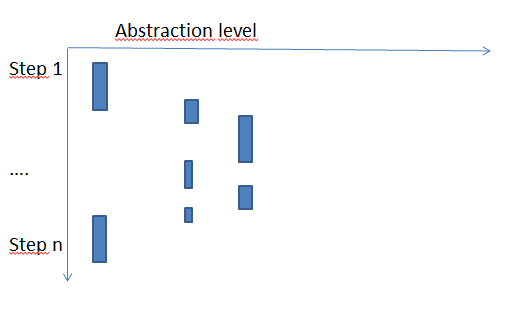
\includegraphics{Bilder/Rule1Abstraction.png}
\caption[Diagramm showing the result when applying rule 1]{Diagramm showing the result when applying rule 1}
\label{picture:rule1abstraction}
\end{figure}


\begin{figure}
\centering
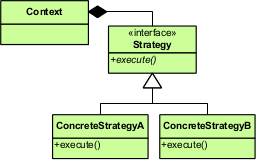
\includegraphics{Bilder/StrategyPattern.png}
\caption[\acf{UML} diagram of the strategy pattern]{\acf{UML} diagram of the strategy pattern}
\label{picture:strategypattern}
\end{figure}

\begin{figure}
\centering
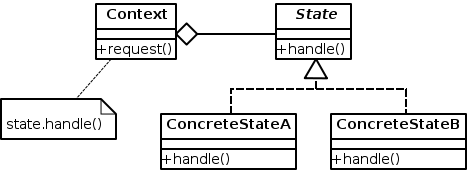
\includegraphics{Bilder/StatePattern.svg.png}
\caption[\acf{UML} diagram of the state pattern]{\acf{UML} diagram of the state pattern}
\label{picture:statepattern}
\end{figure}
%\chapter{Conclusion}

\section{}

\section{}



% ---------------------------- Literaturverzeichnis ----------------------------------------------

\begin{thebibliography}{999999}

\bibitem{bay2008} Bay, Jeff: 
\emph{Object Calisthenics}. \\ In: ThoughtWorks inc. (eds): 
\emph{The ThoughtWorks Anthology. Essays on Software Technology and Innovation}. \\ Raleigh, North California; Dallas, Texas: The Pragmatic Bookshelf, 2008, p. 70--80.

\bibitem{oc2008} ThoughtWorks inc. (eds): 
\emph{The ThoughtWorks Anthology. Essays on Software Technology and Innovation}. \\ Raleigh, North California; Dallas, Texas: The Pragmatic Bookshelf, 2008.

\bibitem{gof} Gamma, Eric; Helm, Richard; Johnson, Ralph; Vlissides,  John:
\emph{Design Patterns. Elements of Reusable Object-Oriented Software}. \\ Amsterdam: Addison-Wesley Longman, 1994.
  
\bibitem{cc} Martin, Robert Cecil:
\emph{Clean Code. A Handbook of Agile Software Craftsmanship}. \\ n.p., Prentice Hall International, 2008.

\bibitem{ref} Fowler, Martin:
\emph{Refactoring. Improving the Design of Existing Code}. \\ Amsterdam: Addison-Wesley Longman, 1999. 

\bibitem{dddbook} Evans, Eric:
\emph{Domain-Driven Design. Tackling Complexity in the Heart of Software}. \\ Amsterdam: Addison-Wesley Longman, 2003. 

\bibitem{cohesionBook} Yourdon, Edward; Constantine, Larry:
\emph{Structured Design: Fundamentals of a Discipline of Computer Program and Systems Design}. Yourdon Press, 1979

\bibitem{telldontaskoriginal} Hunt, Andy; Thomas, Dave:
\emph{The Art of Enbugging} \\ URL http://media.pragprog.com/articles/jan\_03\_enbug.pdf

\bibitem{telldontask} Clean Code Developer:
\emph{Tell, don't ask!} \\ URL http://www.clean-code-developer.de/Tell-don-t-ask.ashx

\bibitem{paperboy} Bock, David
\emph{The Paperboy, The Wallet, and The Law Of Demeter}. \\ URL http://www.ccs.neu.edu/research/demeter/demeter-method/LawOfDemeter/paper-boy/demeter.pdf.

\bibitem{ba.com} Appleton, Brad:
\emph{Introducing Demeter and its Laws}. \\ URL http://www.bradapp.com/docs/demeter-intro.html

\bibitem{jls} Gosling, James; Joy, Bill; Steele, Guy; Bracha, Gilad; Buckley, Axel:
\emph{Java Language Specification}. \\ URL http://docs.oracle.com/javase/specs/jls/se7/jls7.pdf

\bibitem{eclipseDocu} The Eclipse Foundation: 
\emph{Eclipse documentation - Eclipse Kepler}. \\ URL http://help.eclipse.org/kepler/index.jsp.

\bibitem[Wikipedia]{wiki} Wikipedia. The Free Encyclopedia. \\ URL http://www.wikipedia.org. 

\bibitem{about} Haas, Juergen: \emph{Modular Programming}.\\ URL http://linux.about.com/cs/linux101/g/modularprogramm.htm.

\bibitem{twWeb} Thoughtworks inc. \\ URL thoughtworks.com/about-us  (17 November 2013).

\bibitem{eclipseast} Kuhn, Thomas; Thomann, Oliver: Abstract Syntax Tree. \\ URL http://www.eclipse.org/articles/article.php?file=Article-JavaCodeManipulation_AST/index.html.

\end{thebibliography}

% ------------------------------- Anhang ---------------------------------------------------------

\begin{appendix}
\clearpage
\pagenumbering{Roman}						% römische Seitenzahlen für Anhang
\end{appendix}


\end{document}
